% CVPR 2022 Paper Template
% based on the CVPR template provided by Ming-Ming Cheng (https://github.com/MCG-NKU/CVPR_Template)
% modified and extended by Stefan Roth (stefan.roth@NOSPAMtu-darmstadt.de)

\documentclass[10pt,twocolumn,letterpaper]{article}

%%%%%%%%% PAPER TYPE  - PLEASE UPDATE FOR FINAL VERSION
\usepackage[]{cvpr}      % To produce the REVIEW version
%\usepackage{cvpr}              % To produce the CAMERA-READY version
%\usepackage[pagenumbers]{cvpr} % To force page numbers, e.g. for an arXiv version

% Include other packages here, before hyperref.
\usepackage{graphicx}
\usepackage{amsmath}
\usepackage{amssymb}
\usepackage{booktabs}

% --- Add to your preamble ---
\usepackage{amsmath,amssymb}
\usepackage{algorithm}       % floating algorithm environment
\usepackage{algpseudocode}   % pseudocode
\usepackage{caption}
\usepackage{subcaption}      % subfigures if you want side-by-side panels
\usepackage{microtype}       % nicer typography
\usepackage{tcolorbox}       % optional: to highlight small notes

\usepackage{float}
\usepackage{placeins}   % provides \FloatBarrier
\usepackage{ifthen}     % for conditional includes
\usepackage{etoolbox}   % safer if-then helpers (optional)

% ----------------------------


% It is strongly recommended to use hyperref, especially for the review version.
% hyperref with option pagebackref eases the reviewers' job.
% Please disable hyperref *only* if you encounter grave issues, e.g. with the
% file validation for the camera-ready version.
%
% If you comment hyperref and then uncomment it, you should delete
% ReviewTempalte.aux before re-running LaTeX.
% (Or just hit 'q' on the first LaTeX run, let it finish, and you
%  should be clear).
\usepackage[pagebackref,breaklinks,colorlinks]{hyperref}


% Support for easy cross-referencing
\usepackage[capitalize]{cleveref}
\crefname{section}{Sec.}{Secs.}
\Crefname{section}{Section}{Sections}
\Crefname{table}{Table}{Tables}
\crefname{table}{Tab.}{Tabs.}


%%%%%%%%% PAPER ID  - PLEASE UPDATE
\def\cvprPaperID{*****} % *** Enter the CVPR Paper ID here
\def\confName{CVPR}
\def\confYear{2022}


\begin{document}

%%%%%%%%% TITLE - PLEASE UPDATE
\title{Federated Learning Beyond Uniform Participation: Probing and Diversity-Aware Client Selection}

\author{
\small{
$Adriano\  De \ Cesare \ (s333044),\  Mattia \  Cappellino\  (s327277), \ Alessia\  Bevilacqua\  (s327984)  
$}
}


\maketitle

%%%%%%%%% ABSTRACT
\begin{abstract}
  Federated Learning (FL) has emerged as a paradigm for training machine learning models across distributed clients without sharing raw data. 
  Despite its promise, FL faces challenges due to statistical heterogeneity (non-IID client data) and system heterogeneity (variable resources and participation). 
  This paper presents a systematic study of these challenges through experiments on CIFAR-100 and Shakespeare datasets, implementing centralized and federated baselines with varying degrees of heterogeneity. 
  We analyze the impact of client participation patterns and non-IID data distributions on FedAvg performance. 
  Finally, inspired by prior work on client selection, we propose two diversity-aware selection strategies: one leveraging label distribution, entropy, and inter-client distance, and another lightweight approach that is probe-informed and fairness-aware, both demonstrating improved convergence in heterogeneous settings. 
The code can be found at our GitHub repository
  \href{https://github.com/Scrivane/AML_project_5}{GitHub: Scrivane/AML\_project\_5}
  
\text Or alternatively at the link\\
\href{https://github.com/Scrivane/AML\_project\_5}{https://github.com/Scrivane/AML\_project\_5}
\end{abstract}


%%%%%%%%% BODY TEXT
\section{Introduction}
\label{sec:intro}
%-------------------------------------------------------------------------
\subsection{Federated Learning and its Challenges}
Federated learning is a machine learning approach where many clients collaboratively train a model under the coordination of a central server \cite{kairouz2021advances}. The main advantage is that the raw data remains on the client devices, preserving privacy and reducing the need to transfer sensitive information. Only model updates are sent to the server.

However, federated learning also introduces new challenges. As the number of participating devices grows, communication between the clients and the server can become a significant bottleneck. Another challenge is that client data, such as that collected from mobile phones, is often non-IID (not independent and identically distributed) and unbalanced, since it depends on how each user interacts with their device.
%-------------------------------------------------------------------------

\subsection{Baselines and personal contributions}

In this paper we analyze the standard FL scenarios, comparing a centralized baseline with a federated one. 
We also study the impact of client participation (uniform vs. skewed) as well as the effects of heterogeneous data distributions on the federated baseline.
Since we noticed that these two aspects are critical for effective federated learning, we then propose two client selection strategies that can mitigate these challenges.


\section{Methodologies}
\label{sec:formatting} 
\paragraph{Datasets.}
We use two datasets to evaluate our methods: CIFAR-100 and Shakespeare.
CIFAR-100 \cite{Cifar} is an image classification dataset consisting of 60,000 32x32 color images in 100 classes, with 600 images.
Shakespeare \cite{Shakespeare} is a text dataset derived from the works of Shakespeare, used for next-character prediction tasks. Each sample is comprised of a text of 80 characters (x), a next character (y) and a label which contains info about the play title and the character name that is telling the line .
\paragraph{Splits.}
In CIFAR-100 examples are already split between train(50000 samples) and test(10000 samples). To get the validation set we randomly sampled 5000 samples from the training set.
 We ended up with 45000 samples for training, 5000 for validation and 10000 for testing.
In Shakespeare, we split using 90\% of the samples for training, 5\% for validation, and 5\% for testing.  
\paragraph{Centralized Baseline.}
We implemented a centralized baseline model for both datasets in order to provide a performance
 reference. 
For CIFAR-100, we adopted a convolutional neural network inspired by the \textbf{LeNet architecture}, consisting in two convolutional layers with ReLU activations and max-pooling operations,
 followed by three fully connected layers. The final layer outputs logits over the 100 classes.
For the Shakespeare dataset, we employed a character-level recurrent neural network which consists of an embedding layer, a two-layer \textbf{Long-Short-Term Memory(LSTM)} with dropout, and a linear output layer with output dimension equal to the vocabulary size. Given a sequence of characters, it predicts the next character at the end of the sequence.

 Training on CIFAR  and on Shakespeare was performed using cross-entropy loss and stochastic gradient descent,
updating parameters via backpropagation .






\paragraph{Federated Baseline - FedAvg.}
For Federated Learning we adopt the FedAvg algorithm \cite{mcmahan2017communication} , in which a central server coordinates distributed clients. The server initializes a global model, transmits it to a subset of clients, and aggregates their locally updated models through weighted averaging. This procedure is repeated across multiple communication rounds. For our experiments, we impose a step budget of 8000 for CIFAR and 2000 for Shakespeare, constraining the product of local steps \(J\) and the number of global rounds.

\paragraph{Label heterogeneity.} To replicate the label heterogeneity of real-world federated learning scenarios, we fixed the number of classes per client, using values of $N_c \in \{1,5,10,50\}$. For Cifar we used class of the images to do the split , for shakespeare we created a custom dataset where class is a character of a play , so we assigned together also same characters from different plays. 

\paragraph{Participation skewness.} To replicate real-world federated learning scenarios, we also analyzed the impact of skewed client participation.
Using a Dirichlet distribution with parameter $\gamma$, we generated non-uniform client participation probabilities. A smaller $\gamma$ value results in a more skewed distribution, where a few clients are selected more frequently than others.


\section{Experiments}
\subsection{Centralized Baselines}

We tested different schedulers for the centralized baseline to find the one that gives the best performance: StepLR, MultiStepLR, ReduceLROnPlateau, ExponentialLR, OneCycleLR,  CosineAnnealingLR and CosineAnnealingWarmRestarts.
The best one turned out to be OneCycleLR for Cifar to get a better result in a few steps and also to get the best result in the end.
We used 500 rounds for Cifar-100 and 50 rounds on Shakespeare because the model was already showing good accuracy and small improvements in both of them.




 \begin{figure}[H]
    \centering
    \begin{subfigure}{0.48\linewidth}
        \centering
        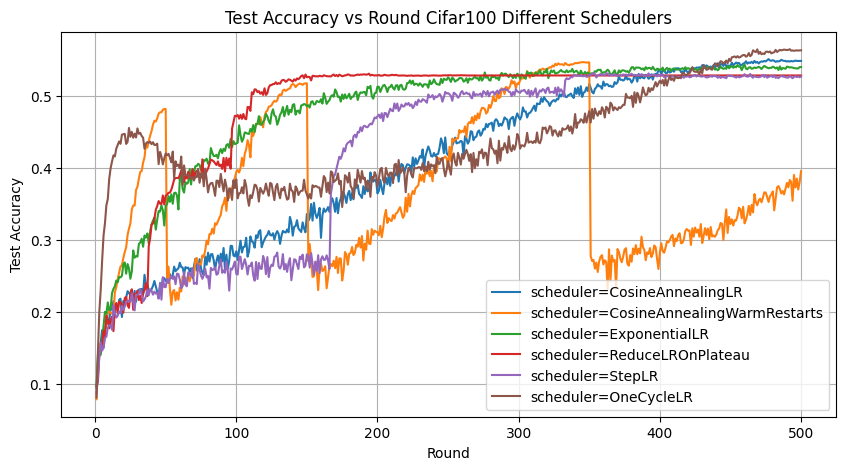
\includegraphics[width=\linewidth]{images/graph_cifar.png}



        \caption{Comparison between different schedulers accuracy on CIFAR dataset.}


        \label{fig:short-a}
    \end{subfigure}
    \hfill
    \begin{subfigure}{0.48\linewidth}
        \centering
        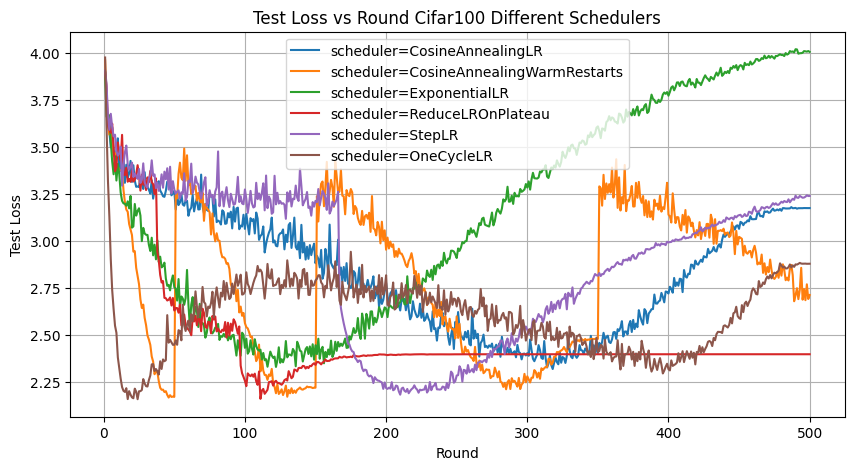
\includegraphics[width=\linewidth]{images/cifar_loss.png}

        \caption{Comparison between different schedulers loss on Shakespeare dataset.}

        \label{fig:short-b}
    \end{subfigure}
    
    \label{fig:cifarBaseline}
\end{figure}

For Shakespeare the best one after 50 rounds turned out to be ReduceLROnPlateau.




 \begin{figure}[H]
    \centering
    \begin{subfigure}{0.48\linewidth}
        \centering
        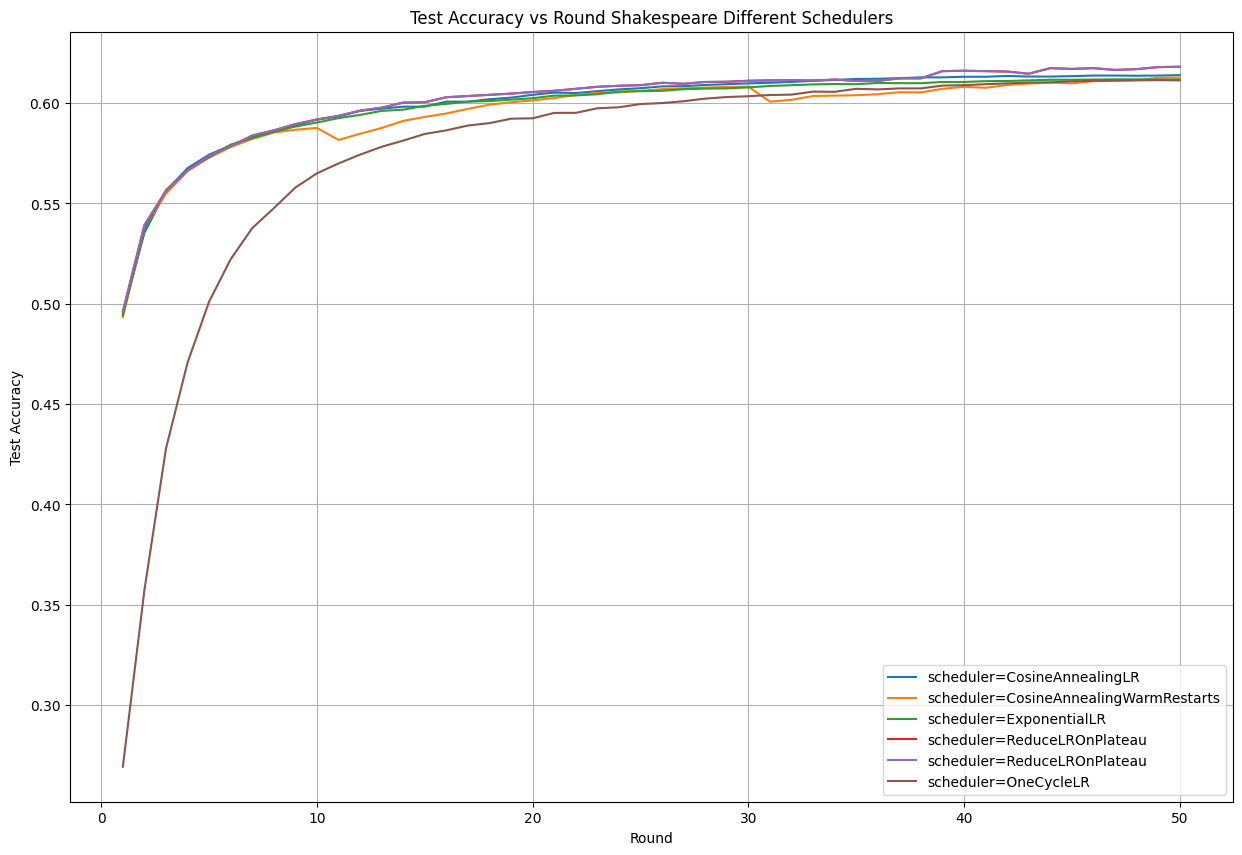
\includegraphics[width=\linewidth]{images/graph_shakespeare.png}


        \caption{Comparison between different schedulers on Shakespeare dataset.}

        \label{fig:short-b}
    \end{subfigure}
    \hfill
    \begin{subfigure}{0.48\linewidth}
        \centering
        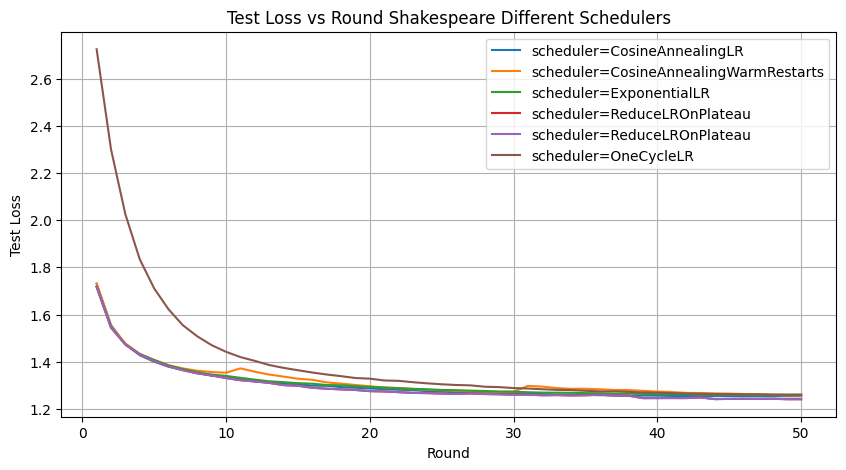
\includegraphics[width=\linewidth]{images/shakespeare_loss.png}

        \caption{Comparison between different schedulers on Shakespeare dataset.}

        \label{fig:short-b}
    \end{subfigure}
    \caption{CIFAR-100 Federated Baseline: Test Accuracy and Test Loss over communication rounds.}
    \label{fig:cifarBaseline}
\end{figure}







There isn't a big difference between different schedulers max accuracy anyway , max difference is around 1\% for shakespeare and 5\% for cifar.


\subsection{Federated Learning Training}
To establish a baseline for the federated setting, we implemented Federated Averaging (FedAvg) [1] on CIFAR-100 with K = 100 IID clients. In each round, 10\% of clients were randomly sampled, each performing 4 local SGD steps before weighted averaging at the server. Training ran for 2000 rounds with a fixed learning rate.

\paragraph{Results.} As shown in Fig.~\ref{fig:cifarBaseline}, FedAvg converges steadily under this configuration. The model reached a \textbf{final test accuracy} of 44.92\%, with a peak of 45.48\% near 2000 rounds. The test loss decreased monotonically during the initial phase before plateauing, suggesting that further improvements could be achieved through optimization strategies such as learning-rate schedules or adaptive client sampling.

 \begin{figure}[H]
    \centering
    \begin{subfigure}{0.48\linewidth}
        \centering
        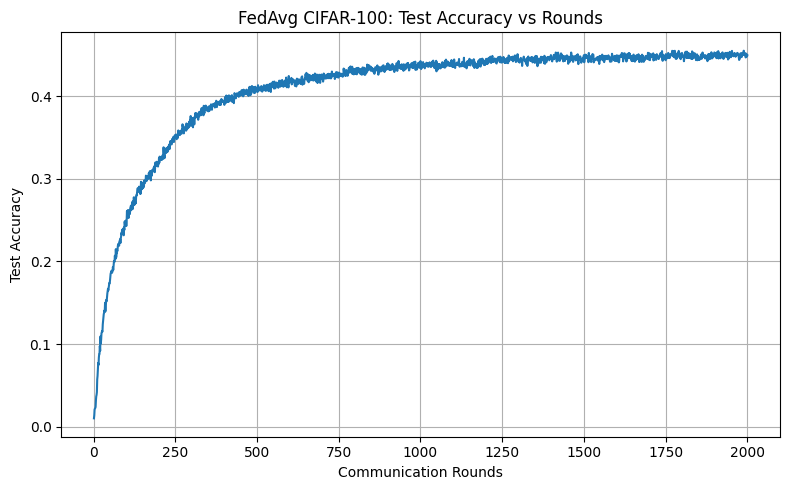
\includegraphics[width=\textwidth]{figs/cifar_fl_baseline_test_acc.png}
        \caption{Test accuracy vs. communication rounds}
        \label{fig:cifarBaselineTestAcc}
    \end{subfigure}
    \hfill
    \begin{subfigure}{0.48\linewidth}
        \centering
        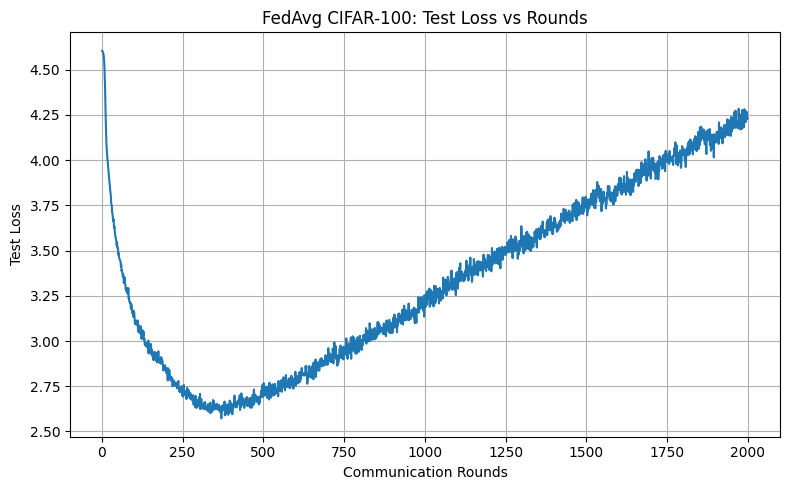
\includegraphics[width=\textwidth]{figs/cifar_fl_baseline_test_loss.png}
        \caption{Test loss vs. communication rounds}
        \label{fig:cifarBaselineTestLoss}
    \end{subfigure}
    \caption{CIFAR-100 Federated Baseline: Test Accuracy and Test Loss over communication rounds.}
    \label{fig:cifarBaseline}
\end{figure}


\subsection{Impact of Client Participation}

To evaluate the effect of client participation on federated learning, we kept the same setup as in the baseline experiments  and varied the client sampling scheme.

\paragraph{Dirichlet-skewed sampling}
Instead of uniform participation, clients were assigned selection probabilities drawn from a \textbf{Dirichlet (\boldmath$\gamma$) distribution}, where smaller $\gamma$ values induce greater skew. We evaluated \textbf{\boldmath$\gamma \in {0.01, 0.1, 0.5, 1, 10}$}.

\paragraph{Results.} As we can see in Fig..~\ref{fig:cifarGamma}, final performance was consistent across all configurations, with test accuracy in the range of $44$--$45\%$. The \textbf{highest result} was obtained with \textbf{\boldmath$\gamma=10$} ($45.56\%$), while even the most skewed case ($\gamma=0.01$) reached a comparable level ($45.02\%$). These findings suggest that FedAvg is relatively robust to different client participation distributions in this setting.

\begin{figure}[H]
    \centering
    \begin{subfigure}{0.48\linewidth}
        \centering
        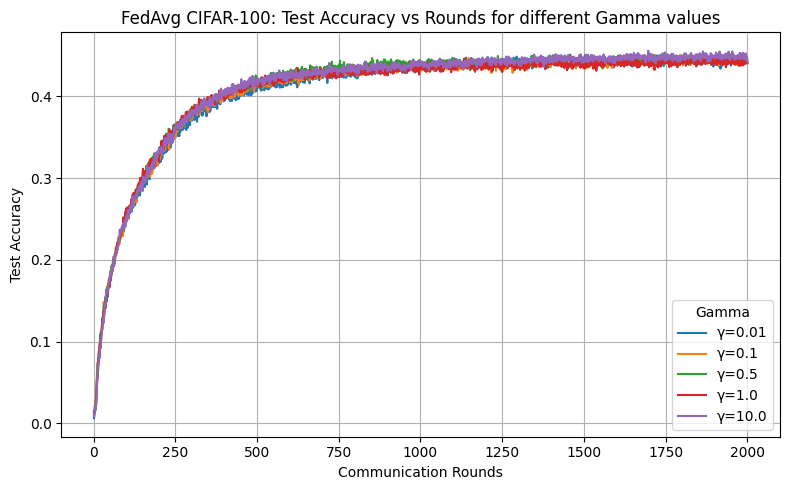
\includegraphics[width=\textwidth]{figs/gamma_values_test_acc.png}
        \caption{Test accuracy vs. communication rounds for different values of $\gamma$ (0.01, 0.1, 0.5, 1, 10).}
        \label{fig:cifarGammaTestAcc}
    \end{subfigure}
    \hfill
    \begin{subfigure}{0.48\linewidth}
        \centering
        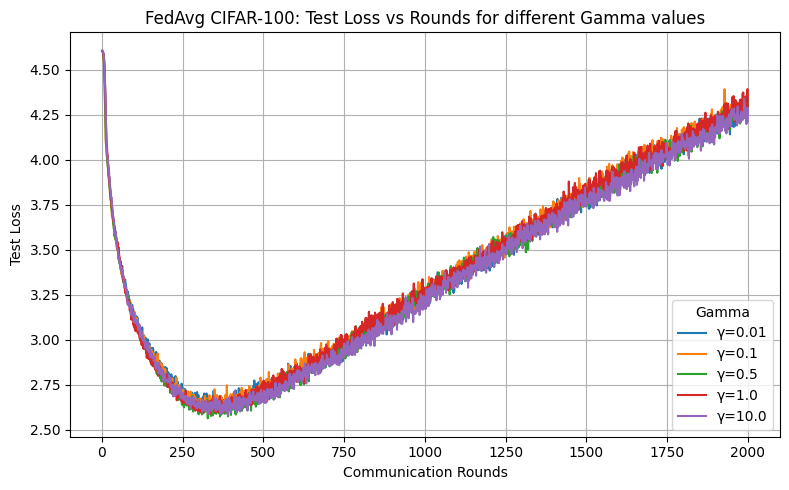
\includegraphics[width=\textwidth]{figs/gamma_values_test_loss.png}
        \caption{Test loss vs. communication rounds for different values of $\gamma$ (0.01, 0.1, 0.5, 1, 10).}
        \label{fig:cifarGammaTestLoss}
    \end{subfigure}
    \caption{CIFAR-100 FedAvg with Skewed Sampling: Impact of varying $\gamma$ on test accuracy and test loss over communication rounds.}
    \label{fig:cifarGamma}
\end{figure}



\subsection{Heterogeneous distribution}
\label{sec:hetero}

\paragraph{Experimental goal and protocol.}
We studied how label heterogeneity across clients affects FedAvg performance. \cite{mcmahan2017communication,hsu2019measuring,hsu2020federated}.Experiments fix the number of clients to \(K=100\) and client fraction \(C=0.1\). We generated several non-IID shardings of the CIFAR-100 training set by constraining the number of distinct labels available to each client: \(N_c\in\{1,5,10,50\}\). \cite{hsu2019measuring,hsu2020federated} An IID baseline (random split into \(K\) shards) is included for comparison. For each sharding we run FedAvg with local epochs \(J\in\{4,8,16\}\). To keep compute comparable, rounds are scaled according to a fixed local-step budget: if \(J_0,R_0\) are the canonical epoch/round pair, then for a new \(J\) we set \(R_{\mathrm{scaled}}=\lfloor (J_0\cdot R_0)/J\rfloor\). \cite{mccandlish2018empirical,you2017large,stich2020local} 










\paragraph{Per-\(N_c\) learning curves (accuracy).}

\begin{figure}[H]
  \centering
  \begin{subfigure}[b]{0.32\linewidth}
    \centering
    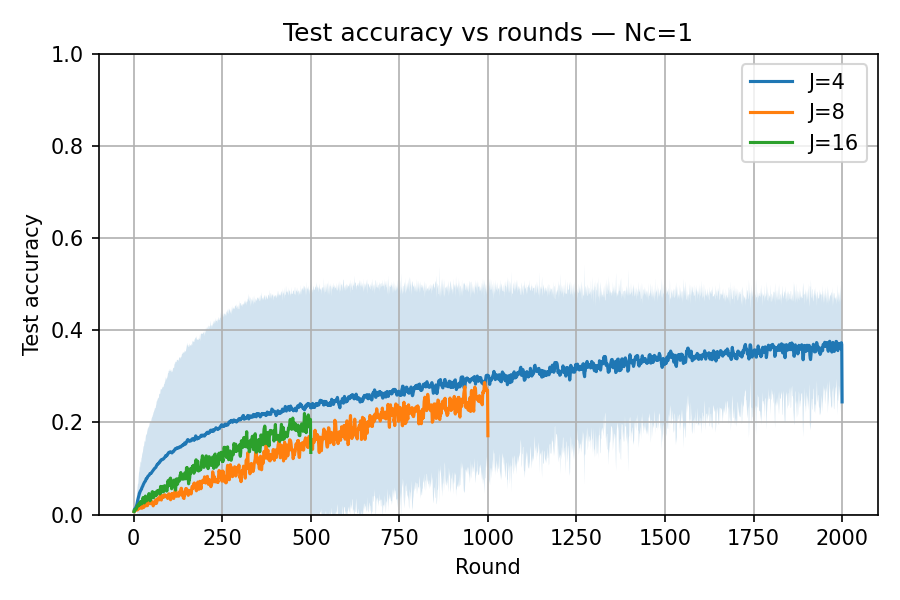
\includegraphics[width=\linewidth]{heter_figs/acc_vs_rounds_Nc_1.png}
    \caption{\(N_c=1\).}
  \end{subfigure}
  \hfill
  \begin{subfigure}[b]{0.32\linewidth}
    \centering
    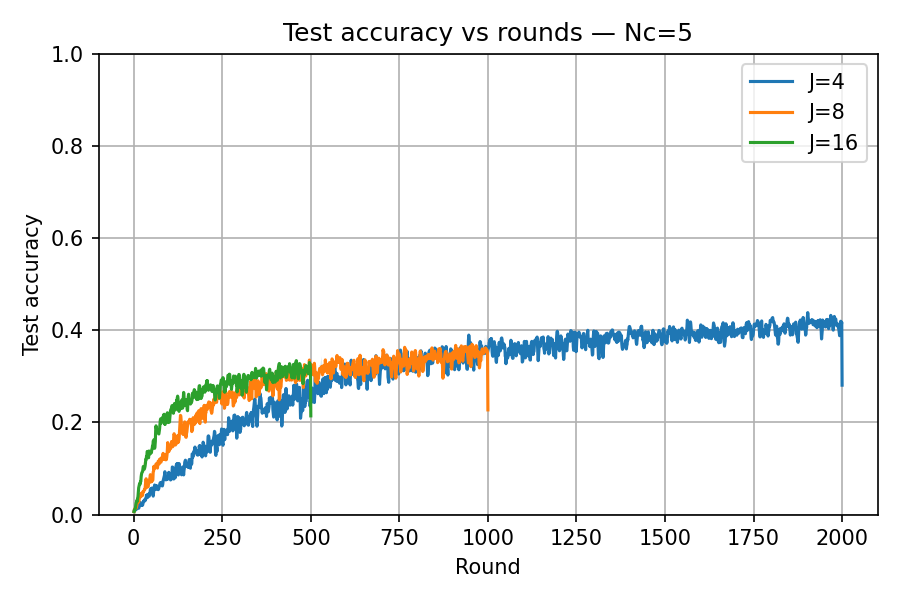
\includegraphics[width=\linewidth]{heter_figs/acc_vs_rounds_Nc_5.png}
    \caption{\(N_c=5\).}
  \end{subfigure}
  \hfill
  \begin{subfigure}[b]{0.32\linewidth}
    \centering
    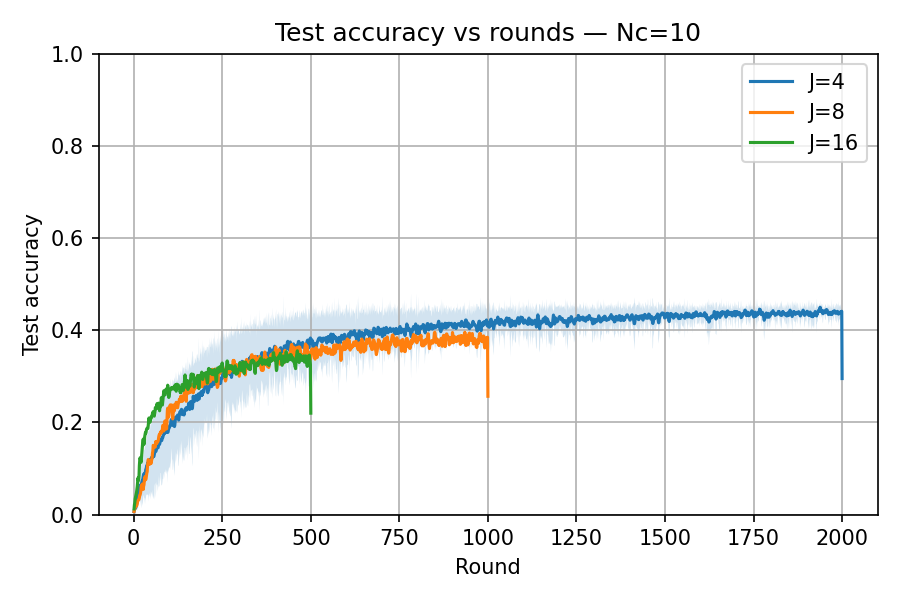
\includegraphics[width=\linewidth]{heter_figs/acc_vs_rounds_Nc_10.png}
    \caption{\(N_c=10\).}
  \end{subfigure}

  \vspace{2mm}

  \begin{subfigure}[b]{0.48\linewidth}
    \centering
    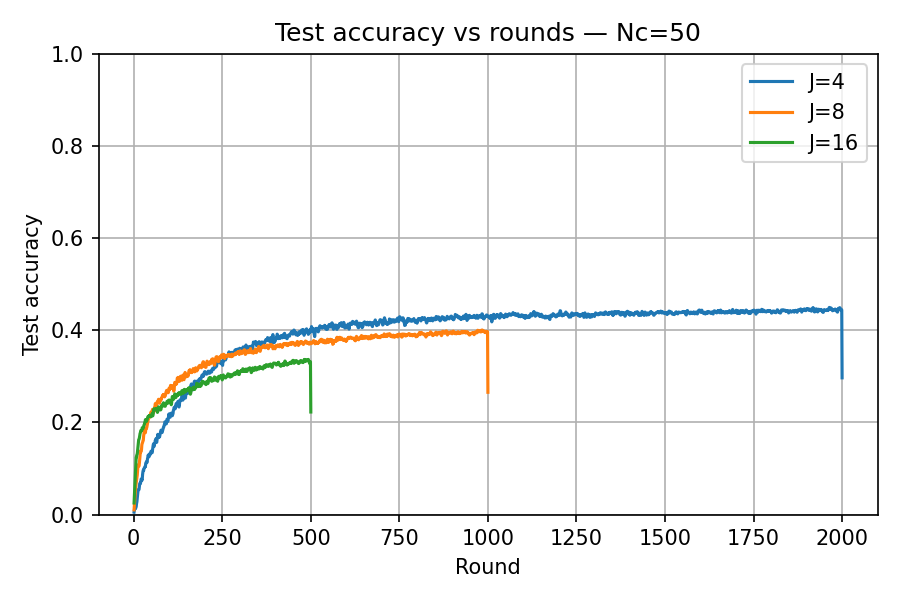
\includegraphics[width=\linewidth]{heter_figs/acc_vs_rounds_Nc_50.png}
    \caption{\(N_c=50\).}
  \end{subfigure}
  \hfill
  \begin{subfigure}[b]{0.48\linewidth}
    \centering
    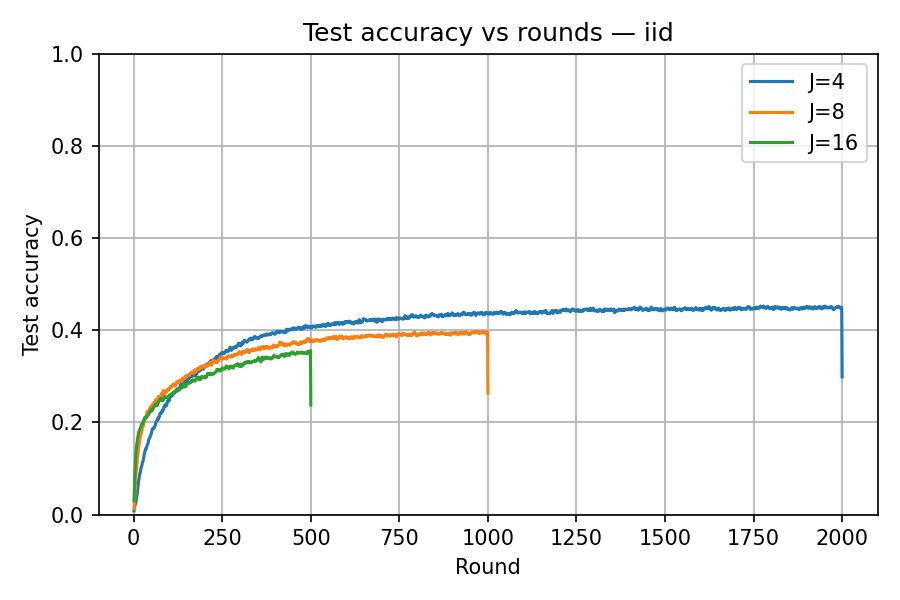
\includegraphics[width=\linewidth]{heter_figs/acc_vs_rounds_iid.png}
    \caption{IID baseline.}
  \end{subfigure}

  \caption{Test accuracy vs rounds separated by label-support \(N_c\). Each plot contains curves for different local epoch budgets \(J\) (\(J=4,8,16\)). Smaller \(N_c\) (more skew) results in slower convergence and lower final accuracy. \cite{hsu2019measuring,li2018federated,karimireddy2020scaffold}}
  \label{fig:hetero-acc-perNc}
\end{figure}

\paragraph{Per-\(N_c\) learning curves (loss).}
\begin{figure}[H]
  \centering
  \begin{subfigure}[b]{0.32\linewidth}
    \centering
    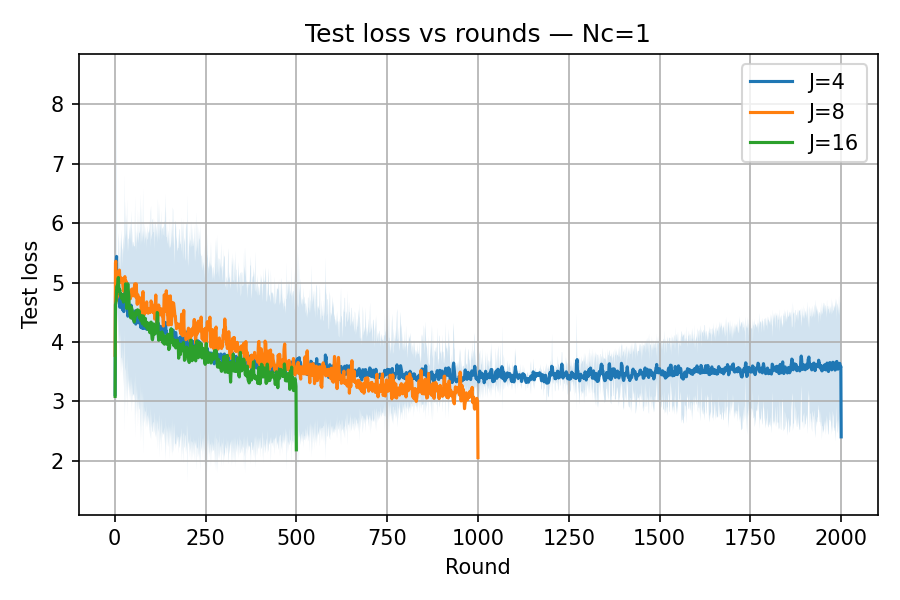
\includegraphics[width=\linewidth]{heter_figs/loss_vs_rounds_Nc_1.png}
    \caption{\(N_c=1\).}
  \end{subfigure}
  \hfill
  \begin{subfigure}[b]{0.32\linewidth}
    \centering
    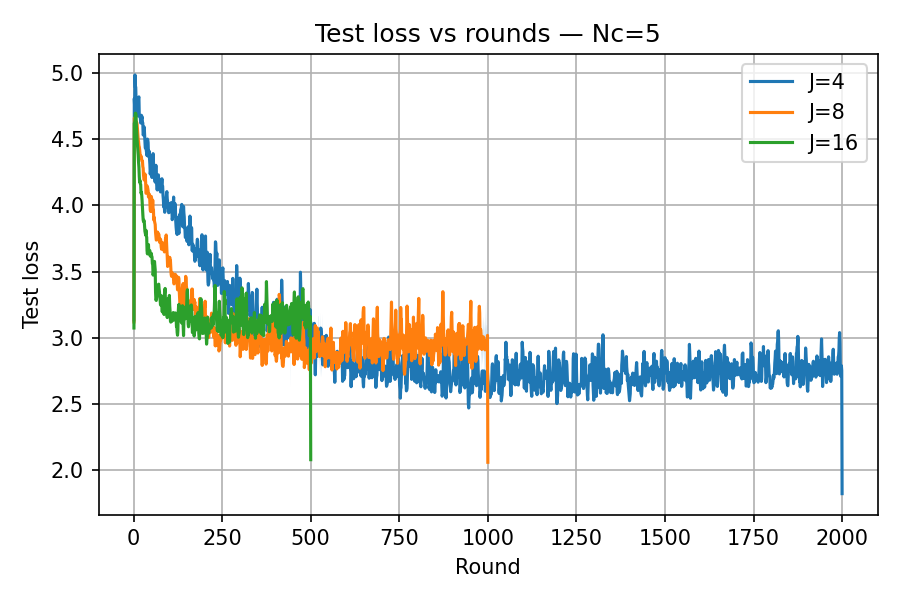
\includegraphics[width=\linewidth]{heter_figs/loss_vs_rounds_Nc_5.png}
    \caption{\(N_c=5\).}
  \end{subfigure}
  \hfill
  \begin{subfigure}[b]{0.32\linewidth}
    \centering
    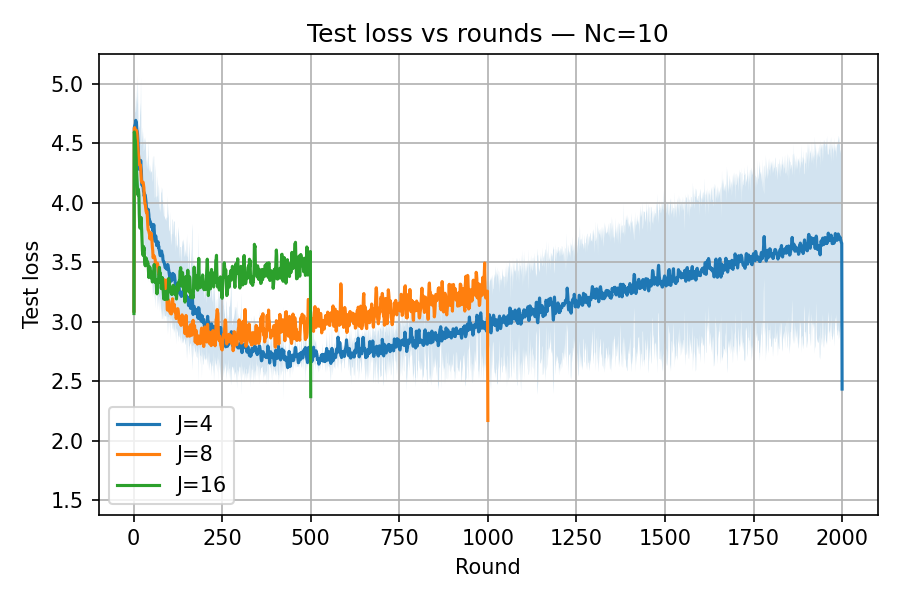
\includegraphics[width=\linewidth]{heter_figs/loss_vs_rounds_Nc_10.png}
    \caption{\(N_c=10\).}
  \end{subfigure}

  \vspace{2mm}

  \begin{subfigure}[b]{0.48\linewidth}
    \centering
    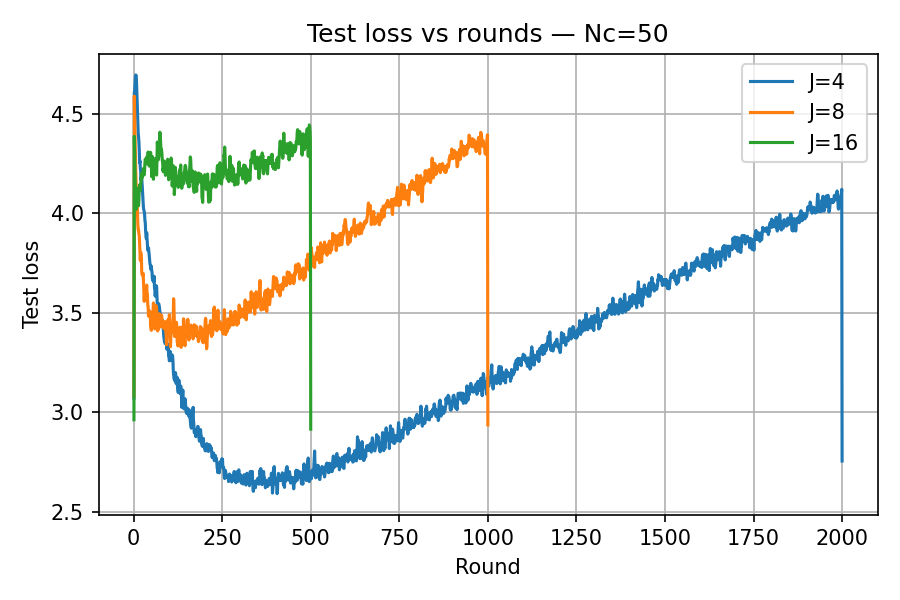
\includegraphics[width=\linewidth]{heter_figs/loss_vs_rounds_Nc_50.png}
    \caption{\(N_c=50\).}
  \end{subfigure}
  \hfill
  \begin{subfigure}[b]{0.48\linewidth}
    \centering
    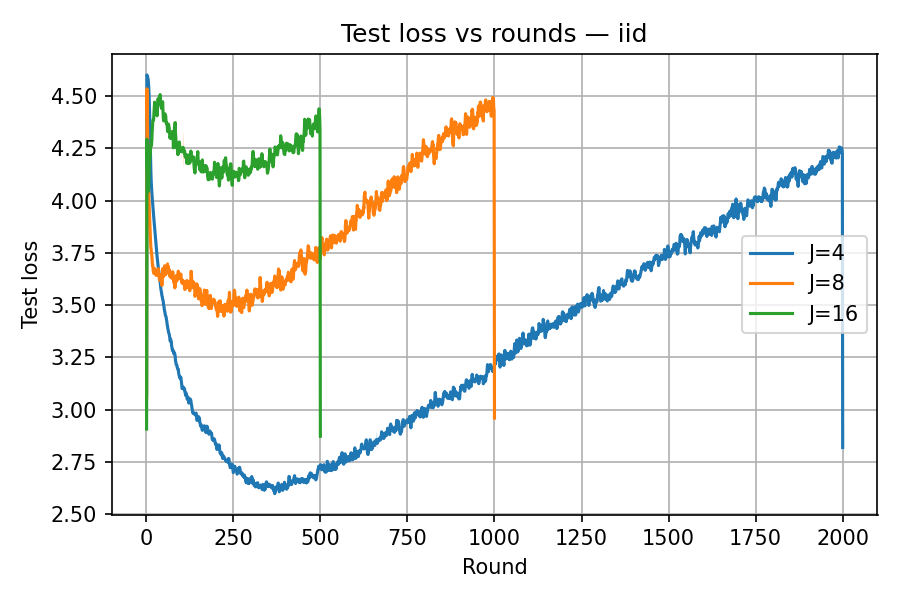
\includegraphics[width=\linewidth]{heter_figs/loss_vs_rounds_iid.png}
    \caption{IID baseline.}
  \end{subfigure}

  \caption{Test loss vs rounds separated by label-support \(N_c\). Loss curves mirror accuracy behavior: greater label skew yields higher loss and noisier trajectories.}
  \label{fig:hetero-loss-perNc}
\end{figure}


\paragraph { Apparent loss-accuracy mismatch}
\label{sec:loss-acc-mismatch}

We observed an empirical mismatch in several CIFAR runs \cite{hsu2019measuring,kairouz2021advances}: around early training the test cross-entropy loss decreases (from $\approx4.5$ to $\approx2.5$) but then gradually increases again (reaching $\approx4.0$) while top-1 test accuracy still slowly rises. This is not a plotting bug — it reflects model calibration and heterogeneity effects. Cross-entropy is sensitive to the predicted probabilities: a small number of highly confident wrong predictions can dominate the average loss, even if many other examples become correctly classified (so accuracy increases). In the federated setting this can arise from selection bias and client drift: the aggregator repeatedly sees updates from fast/majority clients, which drives the model to be overconfident on those classes while performance on rare classes degrades (or becomes overconfidently wrong), increasing average loss.  \cite{karimireddy2020scaffold,li2018federated,nemeth2022client}





\paragraph{Final-summary plots (aggregate across seeds).}
\begin{figure}[H]
  \centering
  \begin{subfigure}[b]{0.48\linewidth}
    \centering
    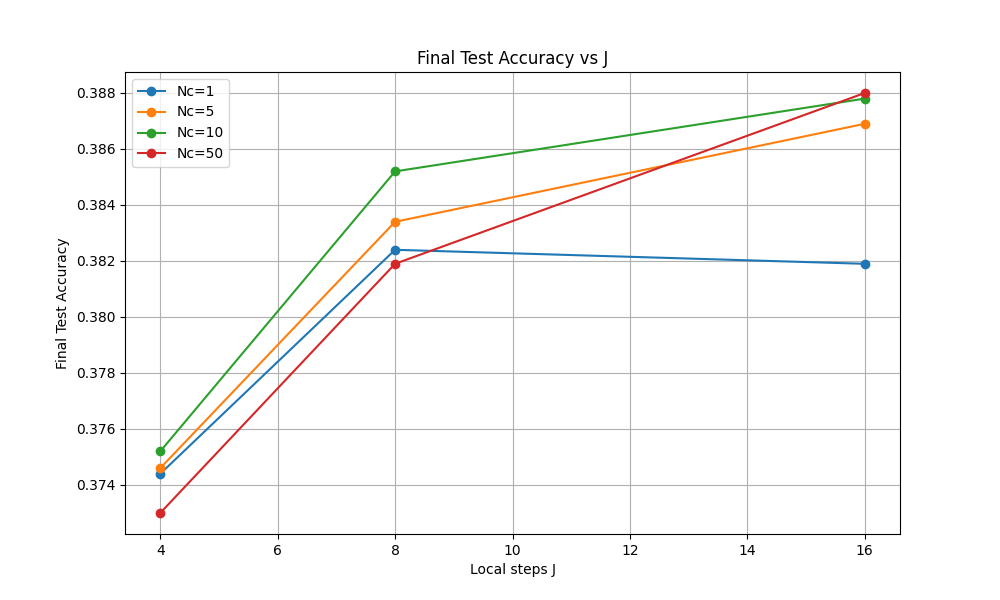
\includegraphics[width=\linewidth]{heter_figs/final_acc_vs_j.png}
    \caption{Final test accuracy vs \(J\) (mean \(\pm\) std).}
    \label{fig:hetero-final-acc}
  \end{subfigure}
  \hfill
  \begin{subfigure}[b]{0.48\linewidth}
    \centering
    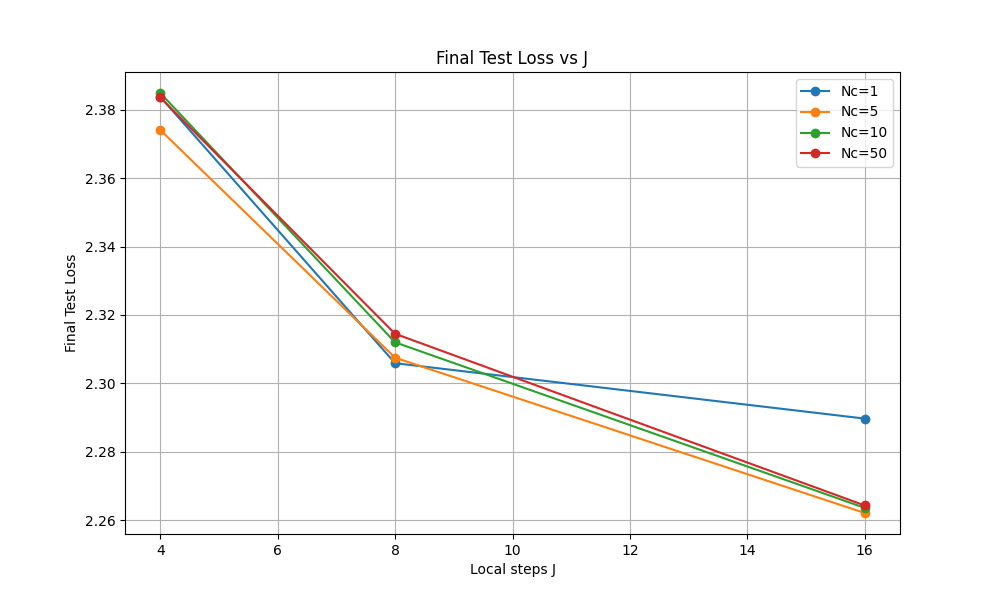
\includegraphics[width=\linewidth]{heter_figs/final_loss_vs_j.png}
    \caption{Final test loss vs \(J\) (mean \(\pm\) std).}
    \label{fig:hetero-final-loss}
  \end{subfigure}
  \caption{Summary plots showing how final accuracy / loss vary with local work \(J\) for each \(N_c\).}
  \label{fig:hetero-final-summary}
\end{figure}

\paragraph{Short interpretation.}
The per-\(N_c\) accuracy and loss plots (Figs.~\ref{fig:hetero-acc-perNc}, \ref{fig:hetero-loss-perNc}) clearly show degradation in both metrics as the per-client label support \(N_c\) decreases. \cite{hsu2019measuring,hsu2020federated} The final-summary plots (Fig.~\ref{fig:hetero-final-summary}) quantify the effect: IID and \(N_c=50\) typically achieve the highest final accuracy and lowest loss; \(N_c=10\) shows moderate degradation; \(N_c=5\) and \(N_c=1\) suffer the largest performance drop and greatest variance. Mechanistically, small \(N_c\) concentrates client data on a few classes, producing biased, high-variance local updates; aggregated updates are therefore noisier and the global model converges more slowly and to a worse point. Increasing \(J\) exacerbates drift for strongly non-iid shardings (not that harmful for IID, but worsen a lot for small \(N_c\)), explaining the differing curves across \(J\).




\paragraph{Results and interpretation.}
There is a notable difference: both accuracy and loss show clear deterioration as \(N_c\) decreases: IID and \(N_c=50\) perform similarly, \(N_c=10\) degrades moderately, while \(N_c=5\) and \(N_c=1\) show the worst final accuracy and highest loss. 

This happens because small \(N_c\) produces many clients whose local data covers very few classes: local objectives become biased, local gradients are high-variance and concentrated on limited features, and aggregation averages noisy updates. This produces slower decrease in loss and lower final accuracy. Increasing local epochs \(J\) amplifies client drift (larger steps away from the global model between synchronizations), which typically helps IID settings (reduced communication overhead) but harms strongly non-iid settings; thus the interaction between \(N_c\) and \(J\) explains the differences seen in both accuracy and loss. \cite{li2018federated,karimireddy2020scaffold}



\paragraph{Heterogeneous distribution on Shakespeare}
\label{sec:shakespeare-hetero}

\paragraph{Experimental setup.}
We repeated the heterogeneous-distribution protocol on the Shakespeare dataset. As for CIFAR-100 we fixed \(K=100\) clients and a participation fraction \(C=0.1\), and compared IID splits with artificial non-IID shardings parameterised by the number of distinct labels per client \(N_c\in\{1,5,10,50\}\). The model is run with local steps \(J\in\{4,8,16\}\) while scaling the number of rounds to keep a fixed local-step budget (500, 250, 125 global rounds respectively for \(J=4,8,16\)). The evaluation metric is top-1 accuracy for next-token prediction.\cite{Shakespeare,kairouz2021advances}

\paragraph{Observed invariance and immediate diagnosis.}
Contrary to CIFAR-100, the Shakespeare experiments show almost no sensitivity to \(N_c\): across the tested shardings the reported top-1 accuracy converges to roughly \(37\%\!-\!38\%\) and the cross-entropy loss hovers near \(2.3\!-\!2.4\). This near-invariance is not a bug but an expected outcome when the global test distribution is heavily dominated by a small set of frequent tokens. \cite{caldas2019leaf,hsu2020federated} In our case a trivial majority-class predictor (always predict the most frequent next letter) already attains a comparable top-1 score; therefore changes to per-client label support have little effect on the global top-1 metric. In short, the model can achieve the dominant-token baseline regardless of \(N_c\), masking any improvements on rare tokens.

\paragraph{Why this differs from CIFAR-100.}
The CIFAR experiments measure a multi-class image classification problem where class labels are (approximately) balanced in the global test set and improving minority-class performance visibly changes top-1 accuracy and loss. Shakespeare is different for two related reasons: (i) the target distribution for next-letter prediction is highly skewed (few tokens dominate), and (ii) role-based shards retain many of these frequent tokens, so even non-IID partitions expose the aggregator repeatedly to the same high-frequency signals. Consequently (a) global top-1 accuracy is an insensitive summary under this modality, and (b) cross-entropy stabilises around the entropy of the dominant distribution.


\paragraph{Concluding note.}
In summary, Shakespeare does \emph{not} contradict the CIFAR-100 findings: non-IID sharding and larger local work still increase heterogeneity and client drift. However, because the modality and test distribution differ, the standard global summaries (top-1 / mean loss) are less informative .


\begin{figure}[H]
    \centering
    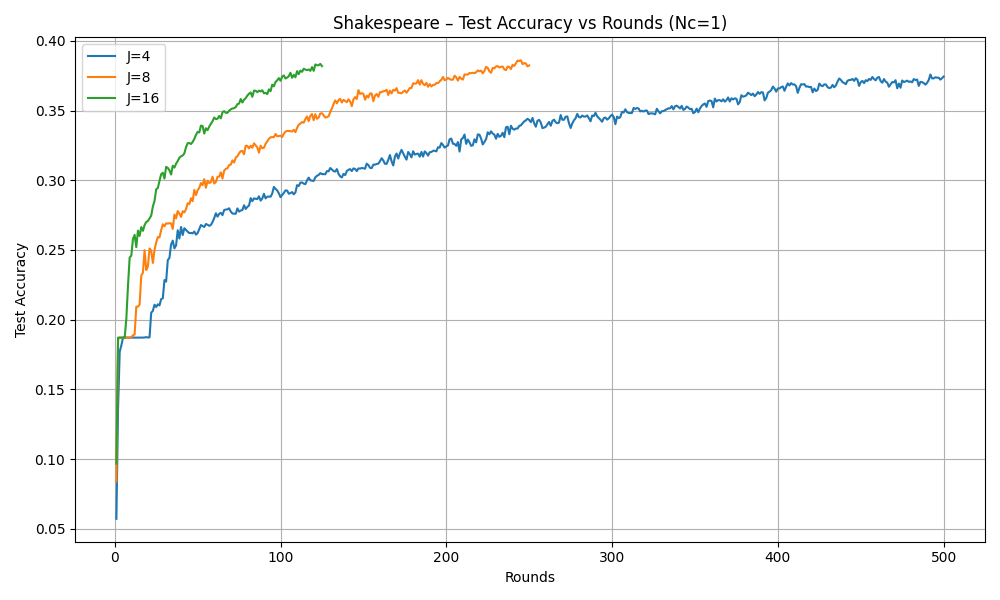
\includegraphics[width=0.45\linewidth]{shak_figs/shakespeare_acc_vs_rounds_1.png}
    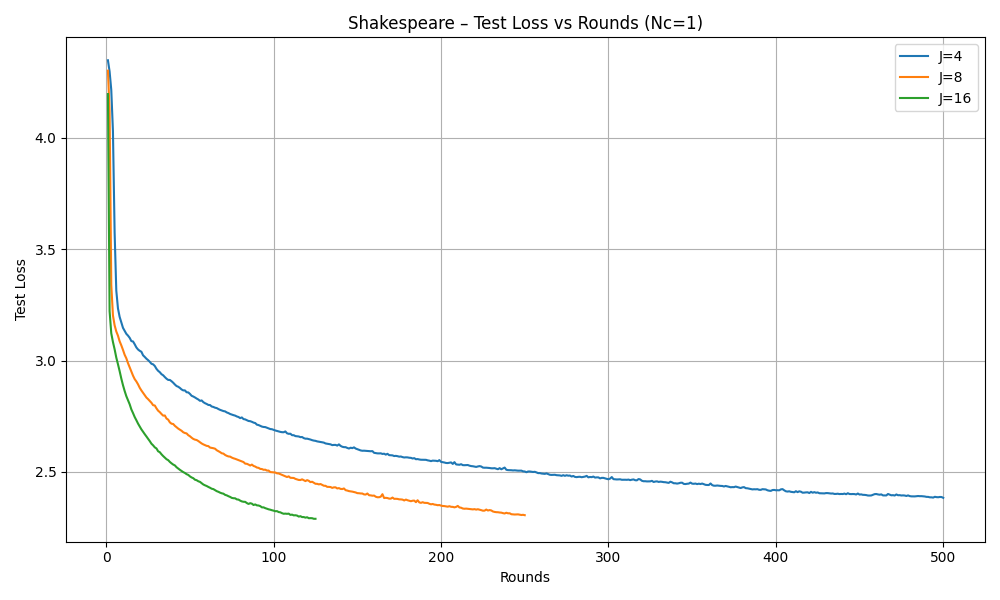
\includegraphics[width=0.45\linewidth]{shak_figs/shakespeare_loss_vs_rounds_1.png}
    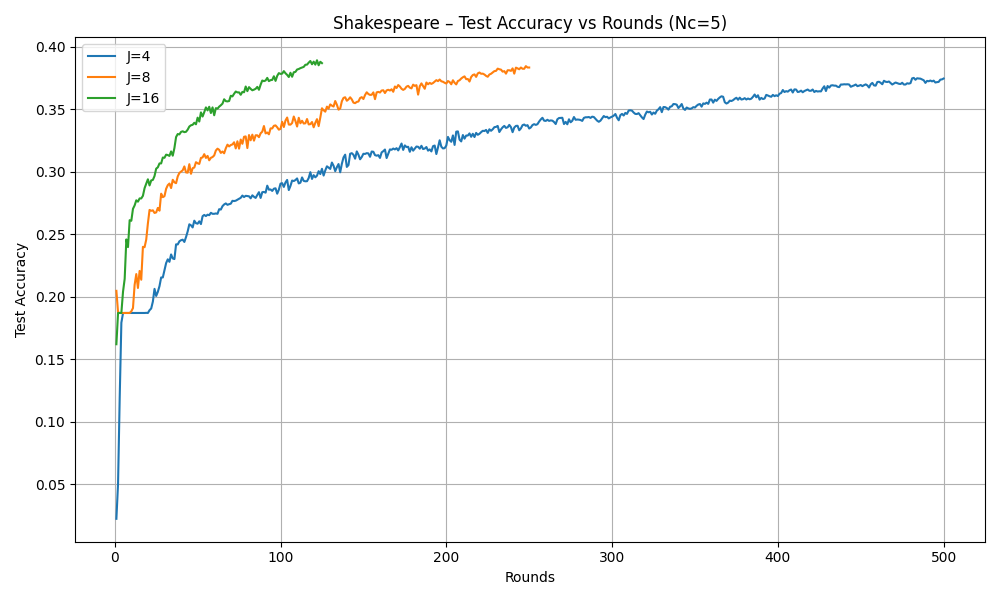
\includegraphics[width=0.45\linewidth]{shak_figs/shakespeare_acc_vs_rounds_5.png}
    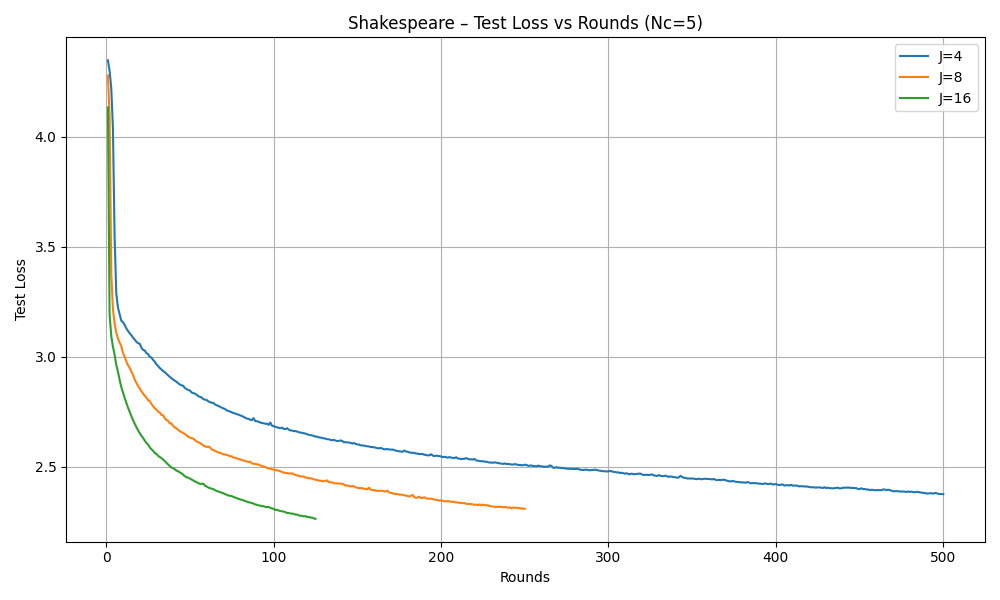
\includegraphics[width=0.45\linewidth]{shak_figs/shakespeare_loss_vs_rounds_5.png}
    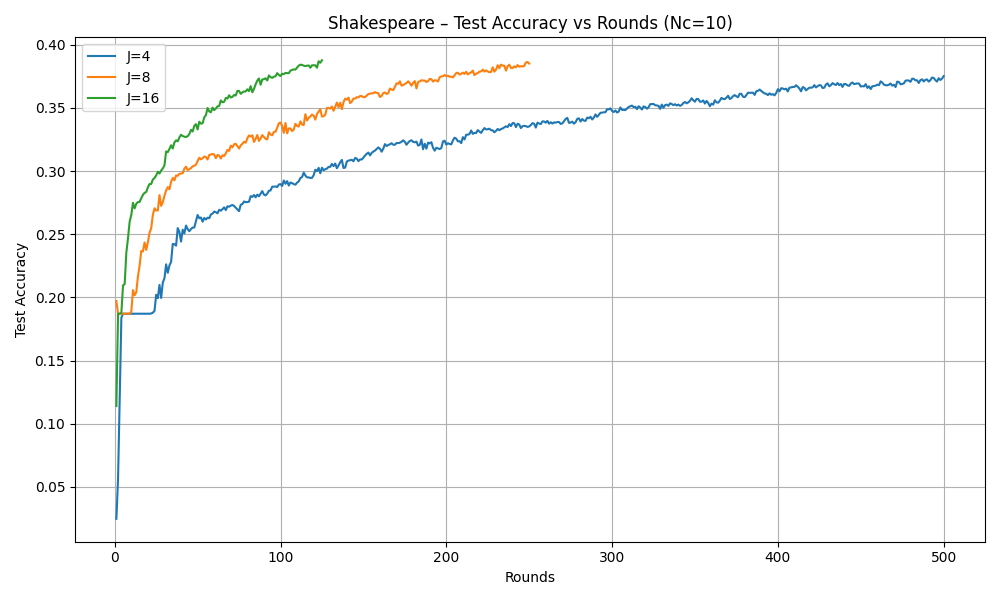
\includegraphics[width=0.45\linewidth]{shak_figs/shakespeare_acc_vs_rounds_10.png}
    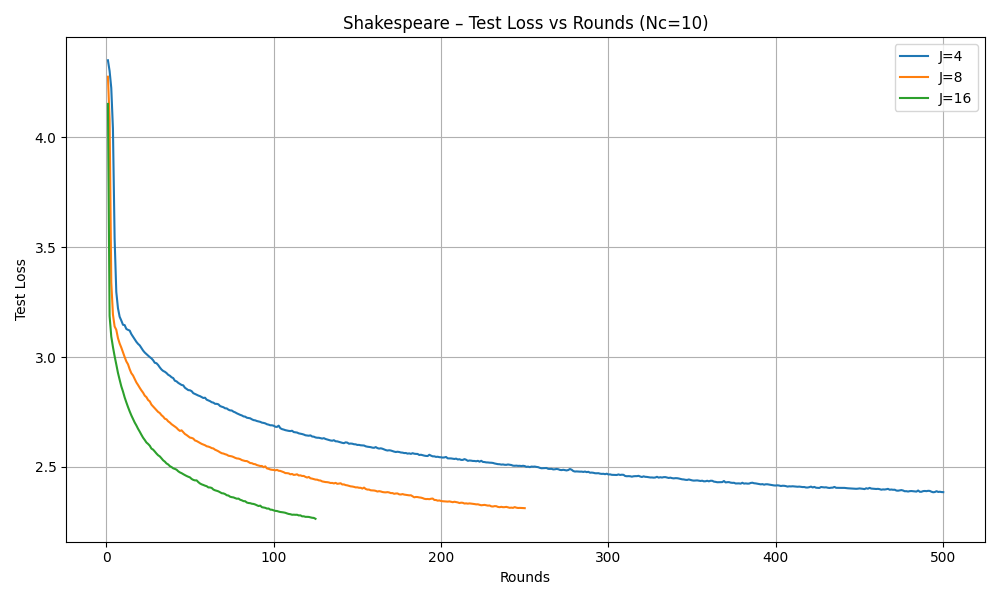
\includegraphics[width=0.45\linewidth]{shak_figs/shakespeare_loss_vs_rounds_10.png}
    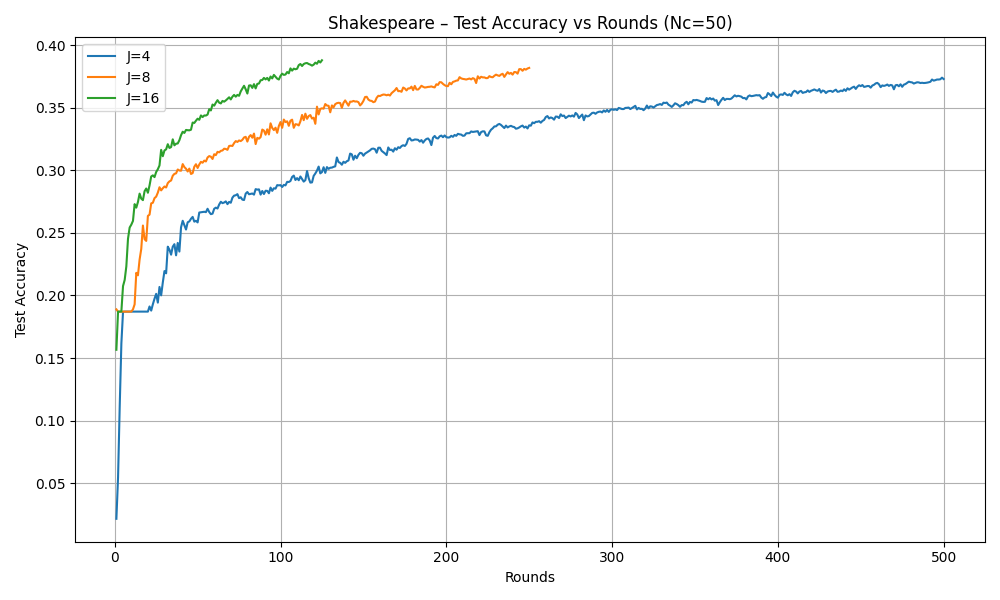
\includegraphics[width=0.45\linewidth]{shak_figs/shakespeare_acc_vs_rounds_50.png}
    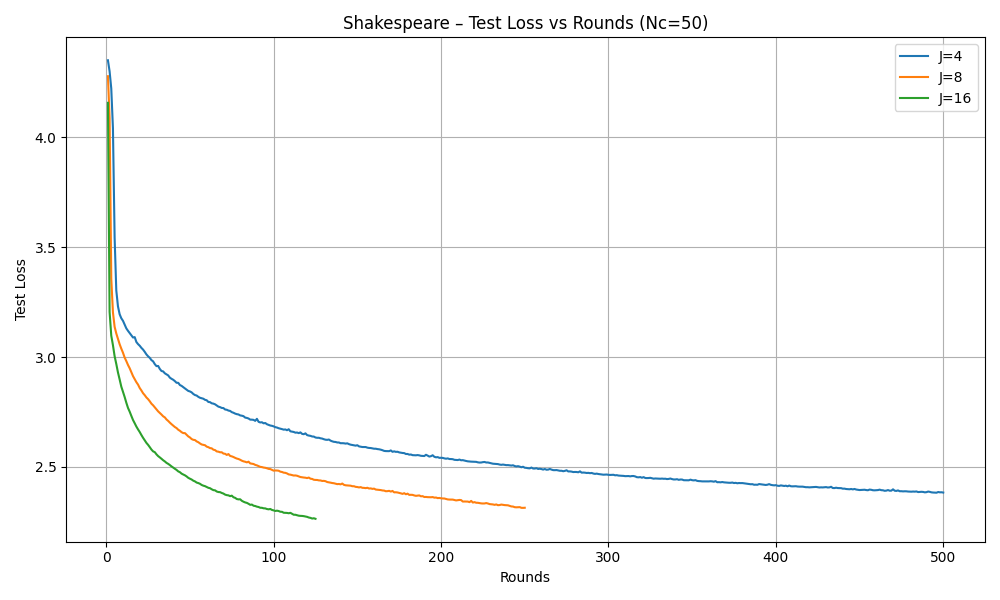
\includegraphics[width=0.45\linewidth]{shak_figs/shakespeare_loss_vs_rounds_50.png}
    
    \caption{Test accuracy and loss over rounds for Shakespeare under different $N_c$ values.}
\end{figure}








\vspace{1mm}








\


















\section{Personal contribution: Client selection under variable client heterogeneity}
\label{sec:personal}

\paragraph{Motivation.}
Federated Learning (FL) typically assumes uniform client participation, but in real deployments clients differ widely in activity and in local data heterogeneity (label support, sample counts). Participation heterogeneity interacts with statistical heterogeneity and can slow convergence, increase variance across clients, and produce unfair outcomes (some clients never contribute meaningfully). In this part of our personal contribution we study client selection: how non-uniform participation affects FedAvg, and whether a lightweight, probe-informed + fairness-aware selection policy can speed early convergence while avoiding long-term starvation of ``weak'' clients. \cite{nemeth2022client,reddi2021adaptive,pfeiffer2023federated} In particular, we explore two selection strategies:
\begin{itemize}
\item\textbf{Probe + fairness hybrid} selection
\item\textbf{Diversity Score} selection
\end{itemize}


\paragraph{Sharder: randomized per-client class support.}
To emulate realistic heterogeneity we introduce a \emph{sampled sharder} that constructs per-client shards by sampling the number of classes per client from a broad distribution, selecting classes with a preference for labels that still have remaining examples, and allocating target examples across the chosen classes. This produces a population that mixes narrow clients (few classes) and broad clients (many classes), increasing variance in per-client updates compared to fixed-$N_c$ schemes commonly used in FL benchmarks.

\subsection{Selection policy: probe + fairness hybrid}
We implement a lightweight hybrid policy combining:
\begin{enumerate}
  \item \textbf{Probe utility:} each round we sample a small candidate pool $C_t$ and run a tiny probe (one or two minibatches) on each candidate to produce a \emph{probe model} $\mathbf{w}_k^{\text{probe}}$. The probe norm is
  \[
    \text{probe\_norm}_k^t = \left\|\mathbf{w}_k^{\text{probe}} - \mathbf{w}^t\right\|_2,
  \]
  which estimates how large an update client $k$ would produce in the near term.
    
  
  \item \textbf{Fairness score:} we compute an inverse-frequency and recency score per candidate to avoid starving clients. Inverse frequency uses $1/(1+\text{count}_k)$ where $\text{count}_k$ is times selected so far; recency is $t - \text{last\_selected}_k$. These components are normalized and blended.
  Both inverse-frequency and recency components are min–max normalized (and so is their blended fairness score) before blending with the normalized probe score; this ensures $\alpha$ mixes comparably-scaled quantities
    
  
  \item \textbf{Blended score and soft exploration:} the final score is a convex blend
  \[
    s_k = (1-\alpha)\,p_k + \alpha\,f_k,
  \]
  where $p_k$ is the normalized probe score, $f_k$ is the fairness score, and $\alpha$ (code: \texttt{beta\_fairness}) trades speed for equity. A small fraction $\epsilon$ of the $m$ client slots is reserved for probabilistic soft exploration using a temperatureed softmax over $s_k$. We also force-select any client not chosen for a long gap (anti-starvation).
    
  
\end{enumerate}
Probe cost is limited by using few minibatches and by reusing the probed model state if that client is selected (so we do not retrain from scratch for the probe work).
    


\paragraph{Algorithms and hyperparameters.}
Local training can use FedProx regularization:
\[
\mathcal{L}_k^{\text{prox}}(\mathbf{w}) = \mathcal{L}_k(\mathbf{w}) + \frac{\mu}{2}\|\mathbf{w}-\mathbf{w}^t\|_2^2,
\]
where $\mu$ penalizes drift from the global model (typical values tested: $\mu\in\{0.01,0.05,0.1\}$). On the server side we also use FedAvgM (server momentum) with velocity $\mathbf{v}^t$:
\[
\mathbf{v}^{t+1} = \beta\,\mathbf{v}^t + \Delta_{\mathrm{agg}}^t,\qquad
\mathbf{w}^{t+1} = \mathbf{w}^t + \eta_s\,\mathbf{v}^{t+1},
\]
We observed that overly large $\eta_s$ together with large per-client deltas can amplify instability. 
In our experiments we apply server momentum and then scale velocity by \texttt{server\_lr} before updating the global model; 
conservative choices ($\eta_s \leq 1.0$, e.g.\ 1.0 or 0.5 depending on clipping) with delta clipping 
(\texttt{clip\_norm} $\approx 10.0$) and moderate momentum ($\beta \in [0.8,0.95]$) improved robustness. 
\textbf{Note:} some earlier runs with \texttt{server\_lr}=0.5 showed instability in our setup and were discarded; 
we treat \texttt{server\_lr}=1.0 with clipping as a more stable baseline.




\paragraph{Analysis: why some clients are strong and others weak.}
A handful of interacting causes explain the observed client disparity:
\begin{itemize}
  \item \textbf{Label support and sample count:} clients with many classes expose the model to more diverse training signal and tend to obtain higher local accuracy and produce larger, more informative updates.
  \item \textbf{Statistical idiosyncrasy:} clients with narrow or unique label mixes can either help (by providing missing labels) or harm (by producing noisy, high-variance updates) global performance.
  \item \textbf {Selection bias and deterministic top-$k$:} a deterministic policy that always picks top probe-norm clients concentrates training on a small subset (fast learners), accelerating short-term progress but starving others. Over time this increases population variance and can reduce final generalization.
  \item \textbf{Optimization interactions:} large per-client deltas combined with high server momentum or large server scaling ($\eta_s$) can create instability (overshoot) unless deltas are clipped or the server learning is conservative.
\end{itemize}

\paragraph{Deterministic top-$k$ behavior (pros and cons).}
Selecting the highest probe norms every round is attractive because it picks clients that promise large immediate improvement (fast convergence in early rounds). However:
\begin{itemize}
  \item \textbf{Positive:} faster early reduction in global loss and fewer rounds-to-threshold for moderate skew.
  \item \textbf{Negative:} deterministic exploitation leads to a bimodal selection frequency distribution (some clients selected very often; many rarely selected) which increases fairness issues and can prevent the model from seeing crucial rare labels. It also increases the chance of unstable aggregation when idiosyncratic clients dominate.
\end{itemize}







\paragraph{Additional results: hyperparameter sweeps and selection statistics}

The plots in this section summarize sensitivity to three selection hyperparameters: the fairness blend weight $\beta$ (code: \texttt{beta\_fairness}), the exploration fraction $\epsilon$, and the softmax temperature $T$ (code: \texttt{temp}). For each hyperparameter we show two side-by-side figures: (left) global test accuracy across rounds, and (right) test loss across rounds.




\label{sec:plots-beta}

\begin{figure}[htbp]  
\noindent\textbf{Sweep: fairness weight \(\beta\).}

  \centering   

  \begin{subfigure}[b]{0.48\linewidth}

    \centering
    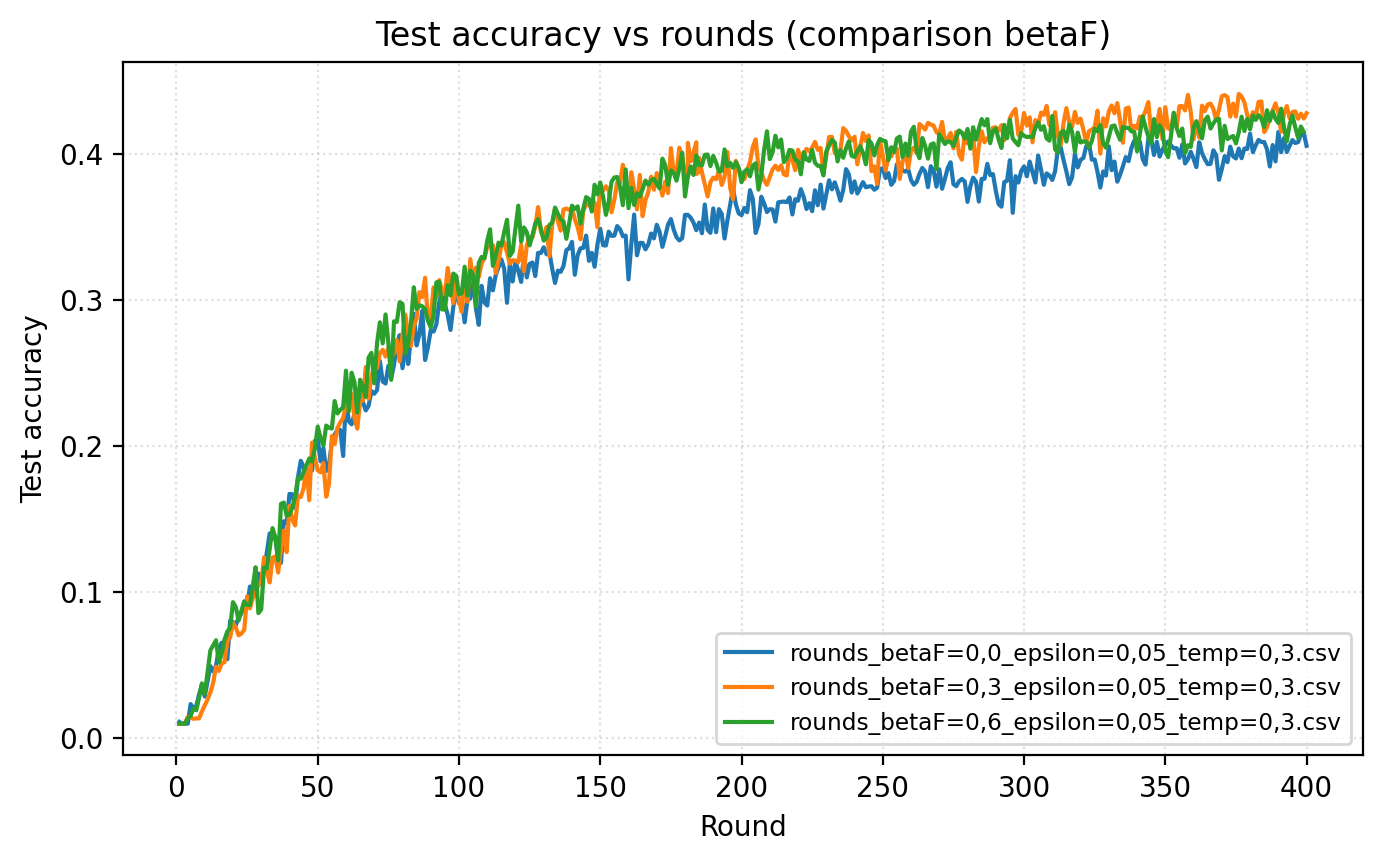
\includegraphics[width=\linewidth]{figs/compare_test_acc_betaF.png}
    \caption{Global test accuracy vs rounds (varying \(\beta\)).}
    \label{fig:beta-acc}
  \end{subfigure}
  \hfill
  \begin{subfigure}[b]{0.48\linewidth}
    \centering
    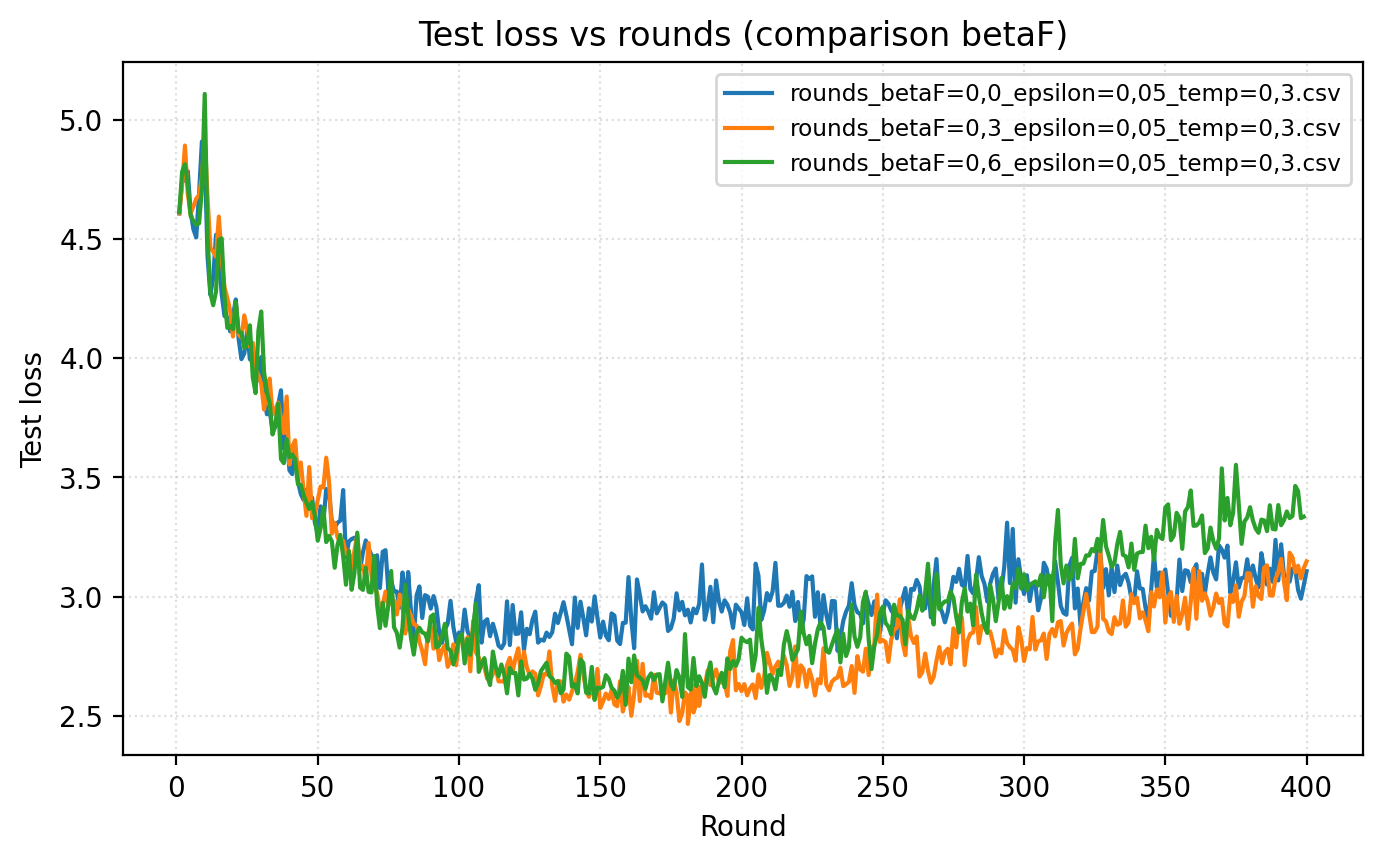
\includegraphics[width=\linewidth]{figs/compare_test_loss_betaF.png}
    \caption{Test loss vs rounds (varying \(\beta\)).}
    \label{fig:beta-loss}
  \end{subfigure}
  \caption{Test accuracy and loss over various fairness weight \(\beta\)  }
  \label{fig:beta-sweep}
\end{figure}
\FloatBarrier




\label{sec:plots-eps}
\begin{figure}[htbp]
\noindent\textbf{Sweep: exploration fraction \(\epsilon\)}

  \centering
  \begin{subfigure}[b]{0.48\linewidth}
    \centering
    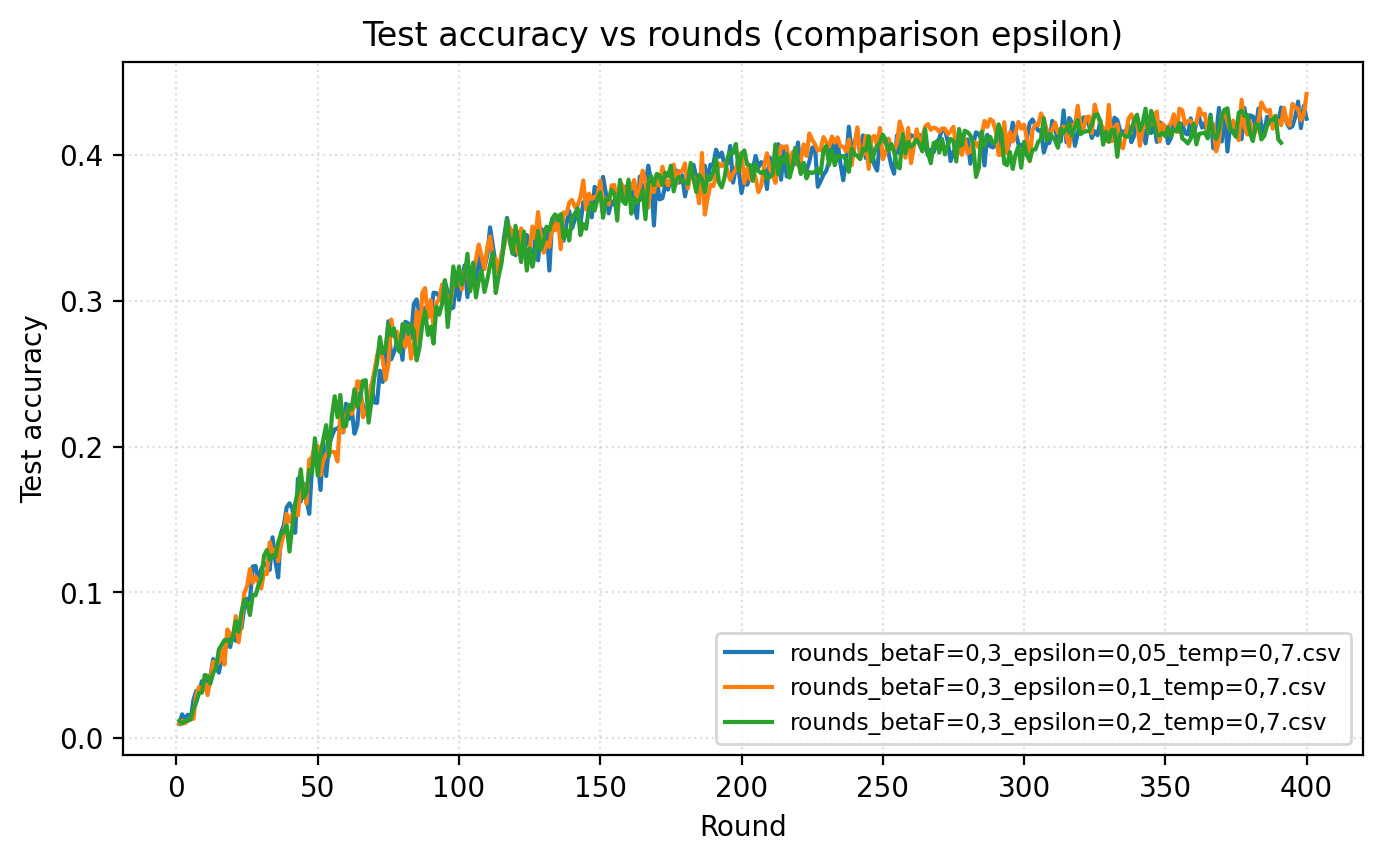
\includegraphics[width=\linewidth]{figs/compare_test_acc_epsilon.png}
    \caption{Global test accuracy vs rounds (varying \(\epsilon\)).}
    \label{fig:eps-acc}
  \end{subfigure}
  \hfill
  \begin{subfigure}[b]{0.48\linewidth}
    \centering
    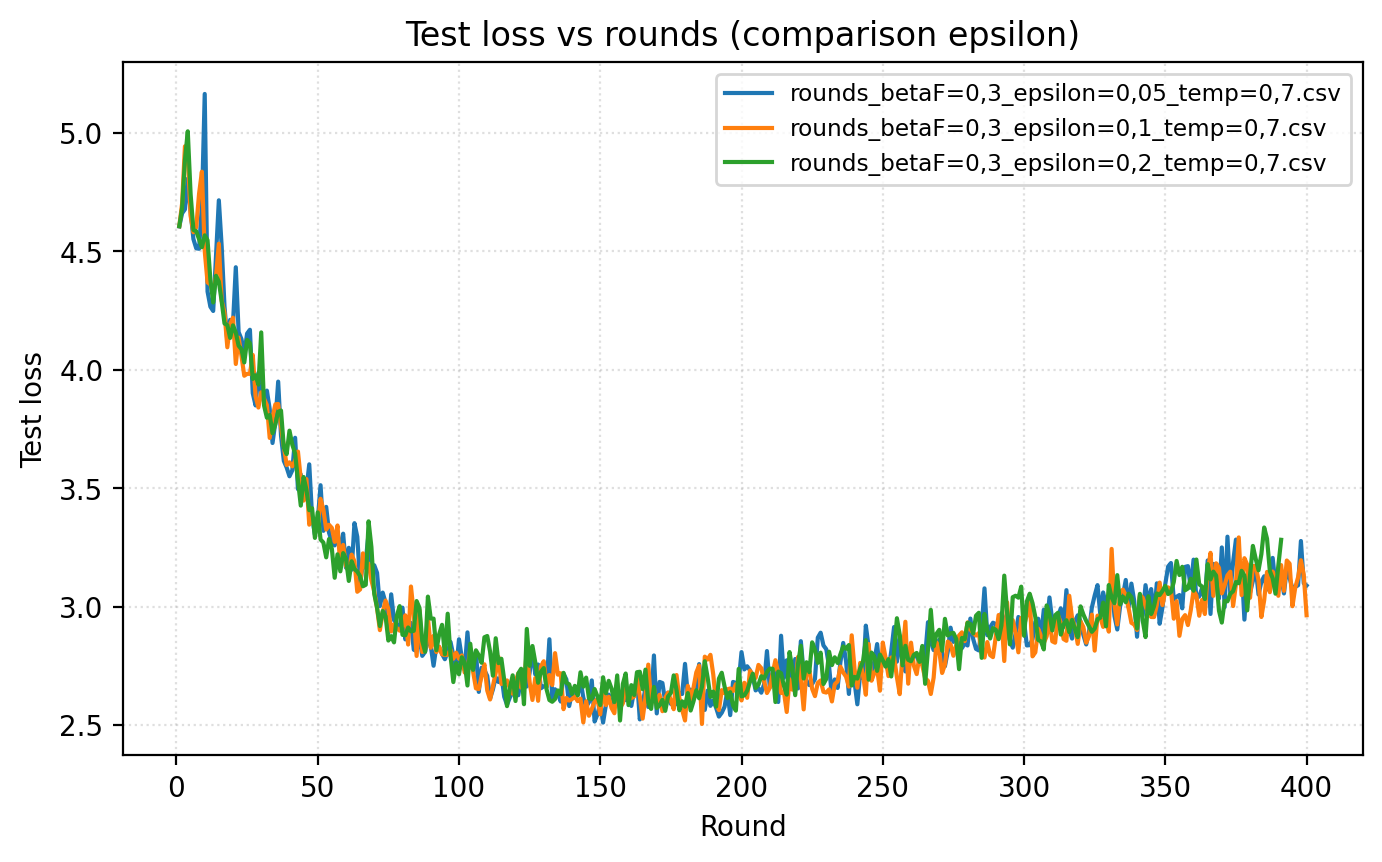
\includegraphics[width=\linewidth]{figs/compare_test_loss_epsilon.png}
    \caption{Test loss vs rounds (varying \(\epsilon\)).}
    \label{fig:eps-loss}
  \end{subfigure}
  \caption{Test accuracy and loss over various exploration fraction \(\epsilon\).}
  \label{fig:eps-sweep}
\end{figure}
\FloatBarrier



\label{sec:plots-temp}
\begin{figure}[htbp]
\noindent\textbf{Sweep: softmax temperature \(T\)}

  \centering
  \begin{subfigure}[b]{0.48\linewidth}
    \centering
    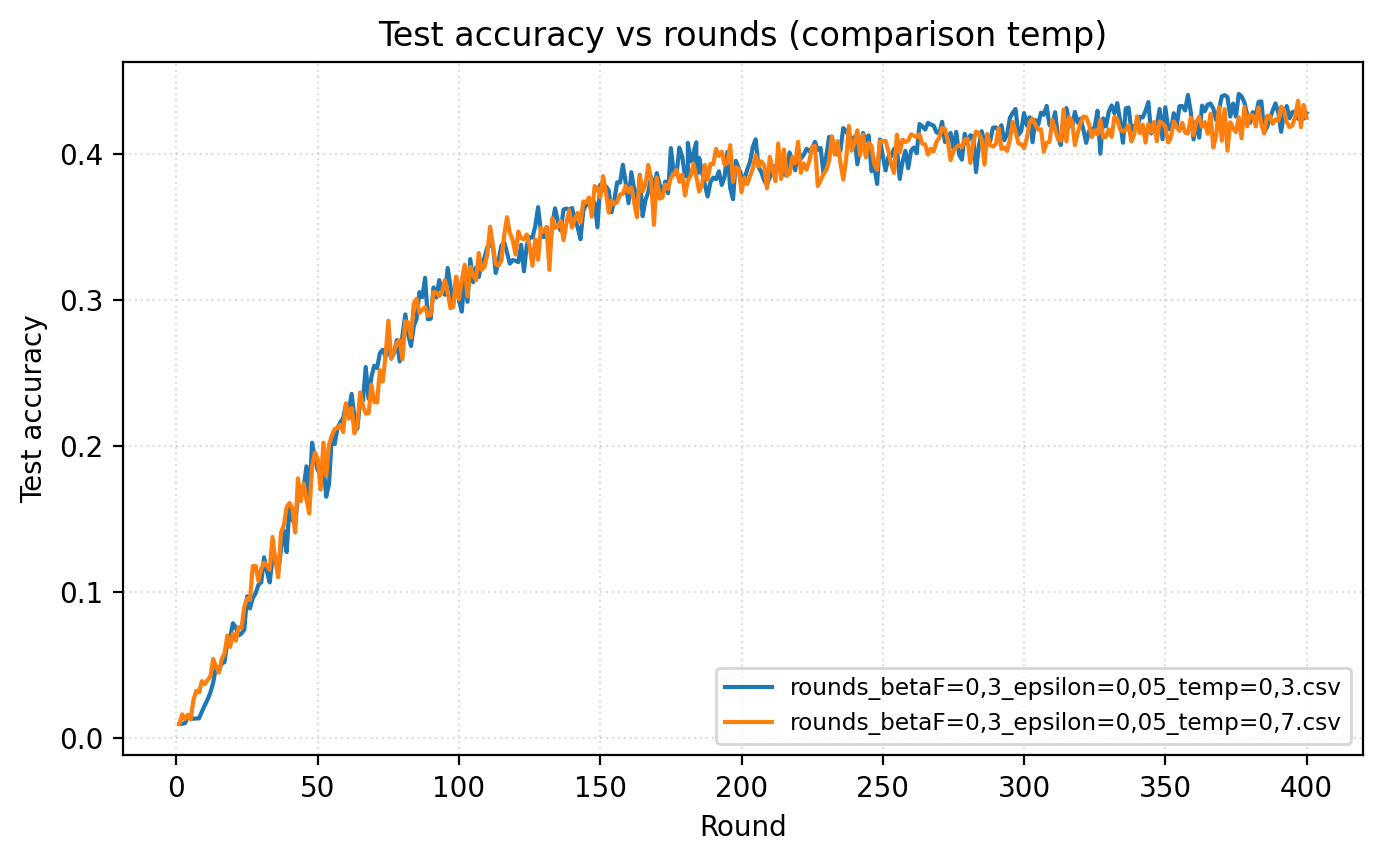
\includegraphics[width=\linewidth]{figs/compare_test_acc_temp.png}
    \caption{Global test accuracy vs rounds (varying \(T\)).}
    \label{fig:temp-acc}
  \end{subfigure}
  \hfill
  \begin{subfigure}[b]{0.48\linewidth}
    \centering
    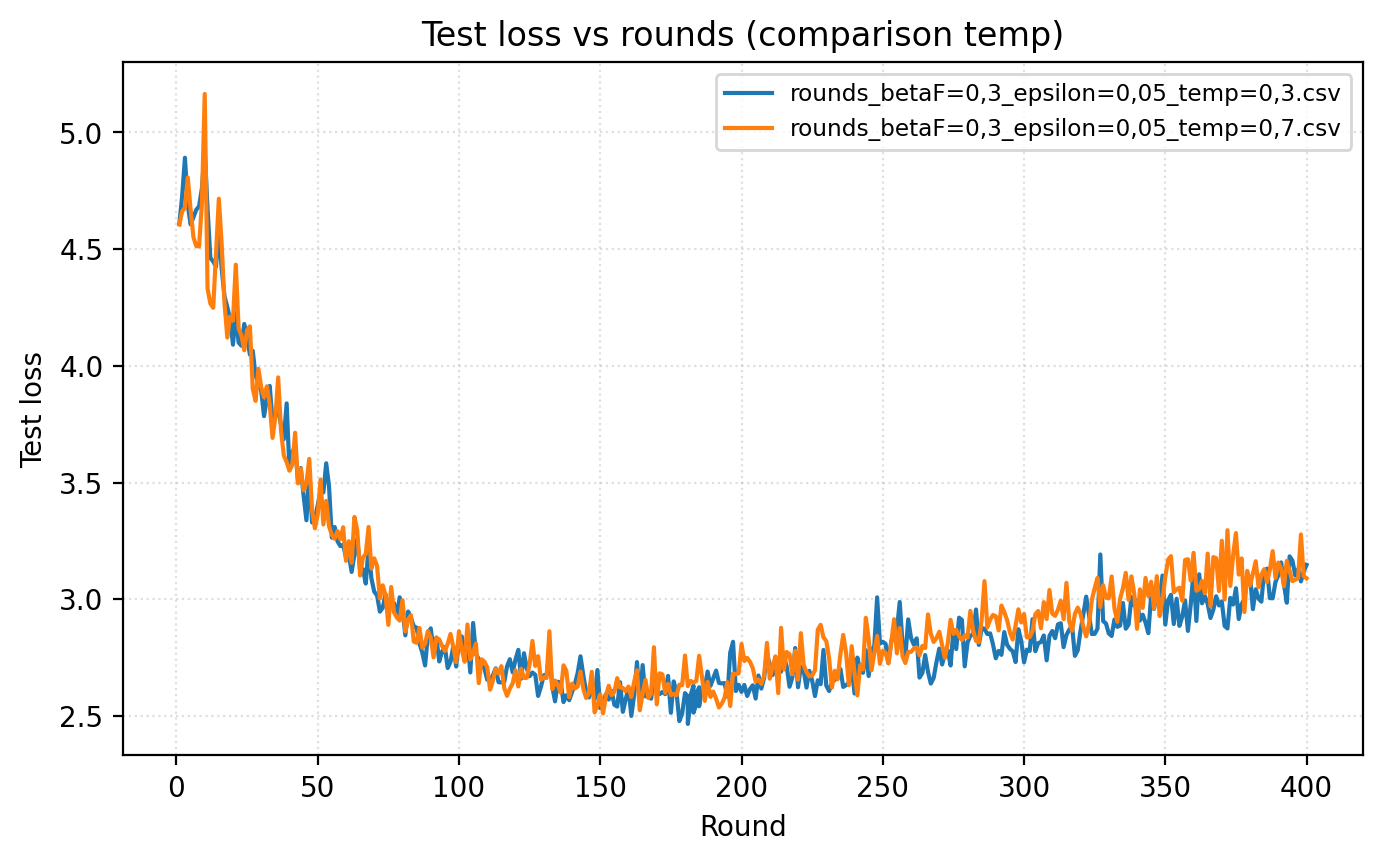
\includegraphics[width=\linewidth]{figs/compare_test_loss_temp.png}
    \caption{Test loss vs rounds (varying \(T\)).}
    \label{fig:temp-loss}
  \end{subfigure}
  \caption{Test accuracy and loss over various sampling temperature \(T\).}
  \label{fig:temp-sweep}
\end{figure}
\FloatBarrier




\label{sec:plots-hist}
\begin{figure}[htbp]
\noindent\textbf{Selection frequency and per-client accuracy histograms}

  \centering
  \begin{subfigure}[b]{0.48\linewidth}
    \centering
    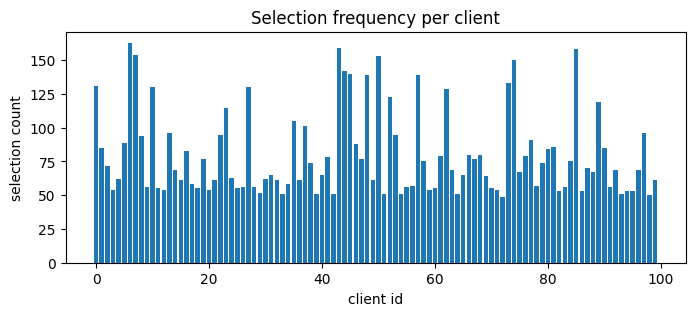
\includegraphics[width=\linewidth]{figs/selection_frequency.png}
    \caption{Client selection frequency (times selected).}
    \label{fig:sel-hist}
  \end{subfigure}
  \hfill
  \begin{subfigure}[b]{0.48\linewidth}
    \centering
    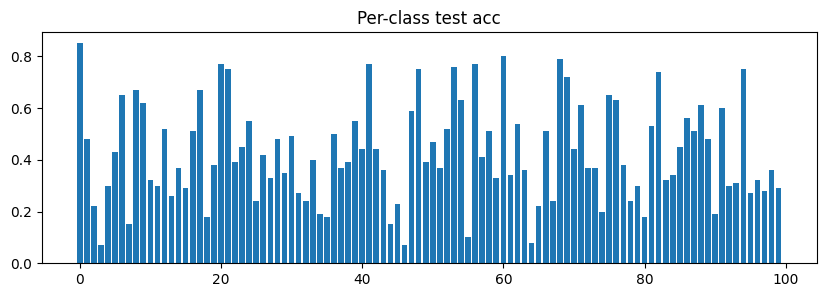
\includegraphics[width=\linewidth]{figs/per_class_test_acc.png}
    \caption{Per-client test accuracy at final round.}
    \label{fig:acc-hist}
  \end{subfigure}
  \caption{(Left) Selection frequency indicates skew and starvation. (Right) Per-client accuracy highlights spread between strong and weak clients.}
  \label{fig:histograms}
\end{figure}
\FloatBarrier











\vspace{1mm}
\noindent\textbf{Takeaway.} Probe-based selection accelerates learning by prioritizing informative clients, but deterministic top-$k$ selection starves many clients and risks instability; blending probe utility with simple fairness and soft exploration yields strong practical gains—faster convergence without starving weak clients.





  





























\subsection{Selection policy: Diversity Score sampling}

\noindent To quantify client diversity, we defined a diversity score that integrates both intra-client and inter-client information. 

\paragraph{Intra-client score.} 
At the intra-client level, we combined two factors: 

\begin{itemize}
    \item \textbf{Structural diversity:} the number of distinct classes present in the local dataset of client \(i\) (\(N_c\));
    \item \textbf{Distributional diversity:} the entropy of the local class distribution (\(H\)), 
    computed through Shannon entropy.
\end{itemize}

\noindent For each client, we represent the local data as a frequency 
vector of length \(C\), where the \(k\)-th entry corresponds to the number of samples belonging 
to class \(k\). Normalizing this vector yields class probabilities \(p_k\), which are then used 
to compute entropy as
\[
H = - \sum_{k=1}^C p_k \log(p_k), 
\quad \text{where } p_k = \frac{n_k}{\sum_{j=1}^C n_j},
\]
\begin{itemize}
\item \(n_k\) = the number of samples belonging to class \(k\) in that client’s local dataset
\item \(\sum_{j=1}^C n_j\) = the total number of samples for that client.

\end{itemize}
Entropy is maximized when all classes present in a client are equally represented, and decreases 
as the distribution becomes more imbalanced.

\noindent These two components were combined into a \textbf{normalized diversity measure} for each client \(i\):
\[
D_i = \lambda \cdot \frac{N_c}{C} + (1 - \lambda) \cdot \frac{H}{\log(C)},
\]
where \(C\) is the total number of classes in the dataset and \(\lambda \in [0,1]\) balances the contribution of structural and distributional diversity.

\paragraph{Inter-client score.} 
To further incorporate inter-client dissimilarity, we extended the definition of the score by computing the mean 
Jensen--Shannon (JS) divergence of client \(i\) with respect to all other clients (\(JS_i\)). 
The final score is then given by:
\[
\text{Score}_i = \alpha \cdot D_i + (1 - \alpha) \cdot JS_i,
\]
where \(\alpha \in [0,1]\) controls the relative importance of intra-client versus inter-client diversity.



\paragraph{Experiments}
In our experiments on diversity score, we evaluate our LeNet-like architecture on CIFAR-100 by varying $\alpha$, which directly controls the degree of statistical heterogeneity between clients. Since this diversity is already established by the sampled sharder and represents the main challenge in federated learning, focusing on $\alpha$ allows us to systematically study its impact on training dynamics while keeping $\lambda$ fixed at 0.5 to balance intra-client diversity. 
\newline To better contextualize the effect of our client-selection method, we also compare results under our heterogeneous sharding scheme (random number of classes per client, with balanced participation) against fixed-$N_c$ baselines from previous experiments, where each client has exactly $N_c$ classes.

\paragraph{Experiments settings.}
CIFAR-100 dataset is divided in: 45k/5k/10k train/val/test split.
FL settings: $K=100$, client fraction $C =0.1$ per round, local epochs $J=4$,  SGDM (LR=0.01, WD=1e-4, momentum=0.9).

\paragraph{Results.}
Across our experiments, we consistently observed the following trends:
\begin{enumerate}    
    \item \textbf{Effect of varying \boldmath$\alpha$.}  
    Performance differences across values of $\alpha$ were modest, yet several patterns emerged. (See Fig.~\ref{fig:testAcc} and ~\ref{fig:testAcc1})  
    \begin{enumerate} 
    \item \textbf{For \boldmath$\alpha=0$}, which relies purely on \textbf{inter-client dissimilarity} (via Jensen–Shannon divergence), the model peaked at 40.7\% but converged to a lower final accuracy of 37.1\%.
    \item \textbf{Intermediate values (\boldmath$\alpha=0.2,0.5$)} that balance inter- and intra-client dissimilarity yielded more stable convergence, with final accuracies of 39.8\% and 40.3\% and peaks at 42.7\% and 42.6\%.  
    \item \textbf{Higher values (\boldmath$\alpha=0.8,1$)}, emphasizing 
    \textbf{intra-client dissimilarity}, yielded no further gains: final accuracies remained in the 40.0 -- 40.9\% range, with slightly higher validation losses suggesting less stable training, a trend mirrored by the final test losses. (Fig.~\ref{fig:testLoss} and ~\ref{fig:testLoss1})
    \end{enumerate} 
    
    \begin{figure}[H]
        \centering
        \begin{subfigure}{0.48\linewidth}
            \centering
            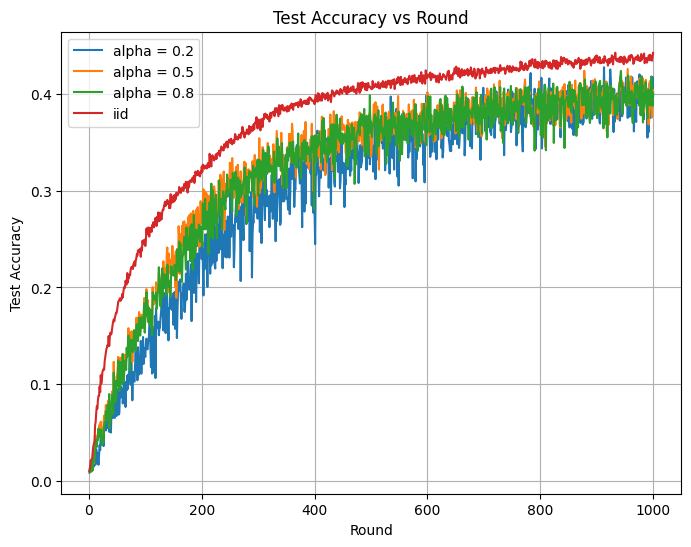
\includegraphics[width=\textwidth]{figs/diversity_test_acc_round_0.2_0.5_0.8.png}
            \caption{Test accuracy vs. communication rounds for different values of $\alpha$ (0.2, 0.5, 0.8).}
            \label{fig:testAcc}
        \end{subfigure}
        \hfill
        \begin{subfigure}{0.48\linewidth}
            \centering
            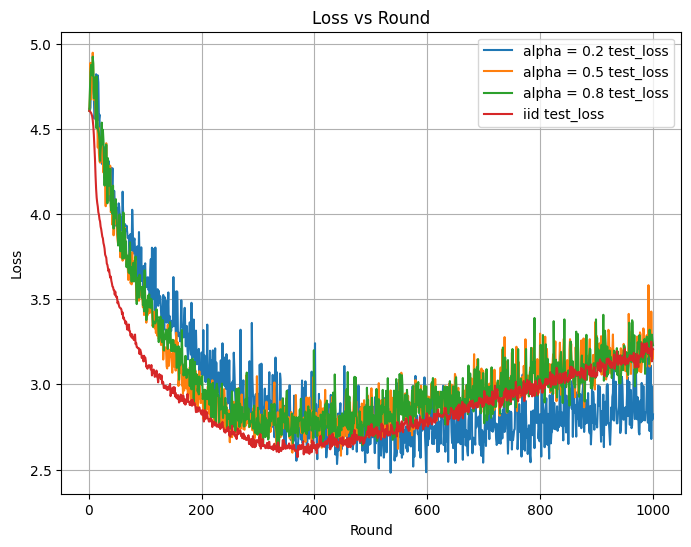
\includegraphics[width=\textwidth]{figs/diversity_test_loss_round_0.2_0.5_0.8.png}
            \caption{Test loss vs. communication rounds for different values of $\alpha$ (0.2, 0.5, 0.8).}
            \label{fig:testLoss}
        \end{subfigure}
        \begin{subfigure}{0.48\linewidth}
            \centering
            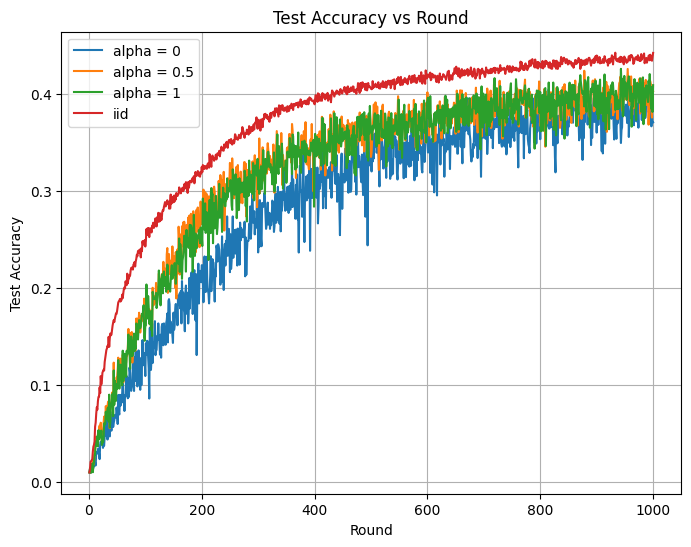
\includegraphics[width=\textwidth]{figs/diversity_test_acc_round_0_0.5_1.png}
            \caption{Test accuracy vs. communication rounds for different values of $\alpha$ (0, 0.5, 1).}
            \label{fig:testAcc1}
        \end{subfigure}
        \hfill
        \begin{subfigure}{0.48\linewidth}
            \centering
            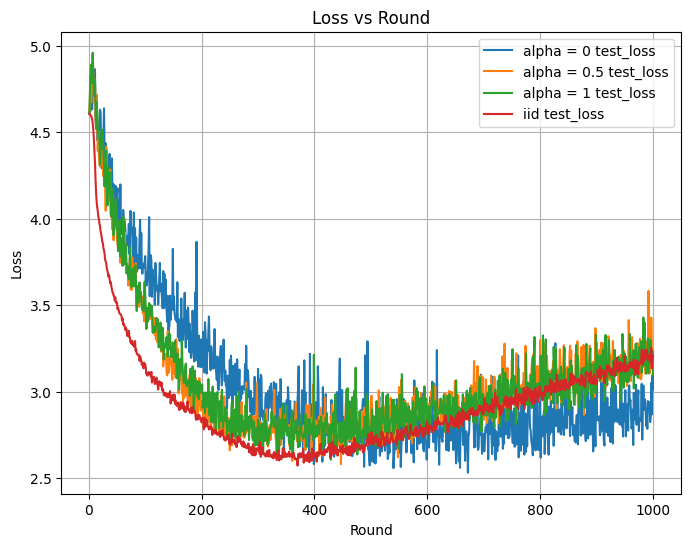
\includegraphics[width=\textwidth]{figs/diversity_test_loss_round_0_0.5_1.png}
            \caption{Test loss vs. communication rounds for different values of $\alpha$ (0, 0.5, 1).}
            \label{fig:testLoss1}
        \end{subfigure}
        \caption{Impact of varying $\alpha$ on test accuracy and test loss over communication rounds.}
        \label{fig:confronto}
    \end{figure}

    Overall, moderate values \textbf{(\boldmath$\alpha=0.2$ -- $0.5$)} provided the \textbf{best trade-off between stability and accuracy}, confirming the value of combining both diversity signals for client selection.
    
    
    
    

    \item \textbf{Comparison with fixed $N_c$ settings.} 
    Experiments using diversity-aware client selection consistently outperformed configurations with low fixed label counts ($N_c=1$ and $N_c=5$), achieved slightly better results than moderate label allocations ($N_c=10$), and remained slightly below the best-performing scenario ($N_c=50$), which approaches the IID baseline. This indicates that selecting clients based on label diversity can effectively mitigate the impact of non-IID distributions while remaining practical for heterogeneous client settings. By adapting naturally to varying label distributions, diversity-based selection balances accuracy and realism: it achieves near-optimal performance without requiring large, uniform label allocations per client, making it suitable for real-world federated learning scenarios.

    \begin{figure}[H]
    \centering
    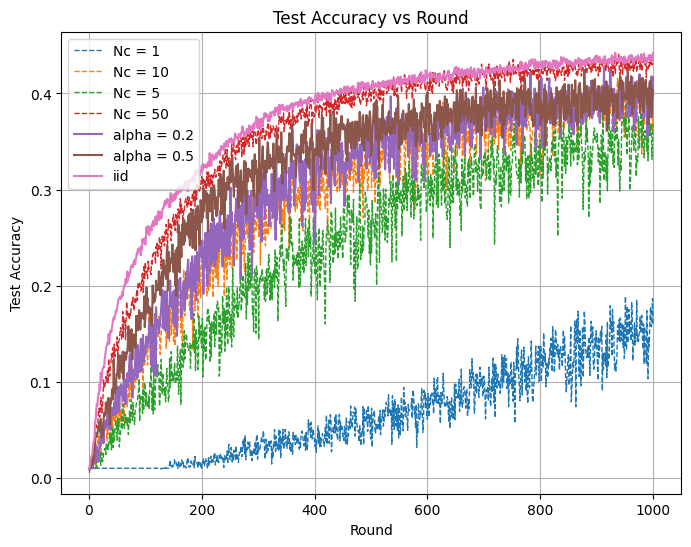
\includegraphics[width=0.6\linewidth]{figs/diversity_score_vs_fixed_Nc.png}
    \caption{Test accuracy of our proposed Diversity Score client selection method compared with the fixed-Nc non-iid baseline.}
    \label{fig:esempio}
    \end{figure}
\end{enumerate}



\section{Conclusion}
In this work, we compared centralized and federated training baselines on CIFAR-100 and Shakespeare, confirming the sensitivity of FedAvg to both data and participation heterogeneity. To address these challenges, we explored client selection strategies. We proposed a Probe + fairness hybrid, which accelerated early convergence while avoiding client starvation, and a Diversity Score policy, which improved stability under heterogeneous splits and skewed participation. Overall, our results show that lightweight, fairness-aware selection can enhance both efficiency and equity, paving the way for more robust deployments of federated learning.














%%%%%%%%% REFERENCES
{\footnotesize
\setlength{\itemsep}{0pt}
\bibliographystyle{ieee_fullname}
\bibliography{egbib}
}








\end{document}


